\documentclass[aspectratio=169]{beamer}
\setbeamertemplate{navigation symbols}{} % don't use navigation tools on slides
% \usetheme{LMT}

\usepackage[utf8]{inputenc}
\usepackage{pdfpc-commands}
\usepackage{multimedia}
\usepackage{listings}
\usepackage{pgfplots}
\usepackage{default}
\usepackage{xcolor}

\newcommand{\parallelsum}{\mathbin{\!/\mkern-5mu/\!}}

\setbeamersize{text margin left=0.6cm,text margin right=0.6cm}
\setbeamercolor{frametitle}{fg=black}
\setbeamercolor{section in toc}{fg=black}
\setbeamertemplate{frametitle}{\color{black}\bfseries\insertframetitle\par\vskip-6pt{\color{gray}\hrulefill}}

\lstset{language=C++,
  basicstyle=\ttfamily,
  keywordstyle=\color{blue}\ttfamily,
  stringstyle=\color{red}\ttfamily,
  commentstyle=\color{green}\ttfamily,
  morecomment=[l][\color{magenta}]{\#}
}

\AtBeginSection[]{
  \begin{frame}{Summary}
    \tableofcontents[currentsection]
  \end{frame} 
}

% refaire les speedup avec du non vide (pour le SIMD)


\begin{document}

\begin{frame}
    \begin{center}
        {\huge High Performance Computing of Power Diagrams}

        \bigskip
        {\large Applications to Semi-Discrete Optimal Transport}
      
        \vfill
        {(MAGA days, November 21, 2019, Hugo Leclerc)}
    \end{center}
\end{frame}

% ---------------------------------------------------------------------------------------
\section*{Introduction}

\begin{frame}
    \frametitle{The world needs power diagrams !}

    \begin{minipage}[c][0.6\textheight][c]{0.5\textwidth}
        Optimal way to transport a density to a set of diracs (equal mass) ? 
        
        \vfill
        Quadratic cost (euclidian distance) $\Rightarrow$ \textit{attributions} are 
            defined by power diagrams.
        
        \vfill
        $x \in$ cell $i$ if $\forall j \neq i$,
         $$|| x - \rho_i ||^2 - \omega_i < || x - \rho_j ||^2 - \omega_j $$
    \end{minipage}
    \kern 0.5cm
    \begin{minipage}{0.45\textwidth}
        \begin{center}
            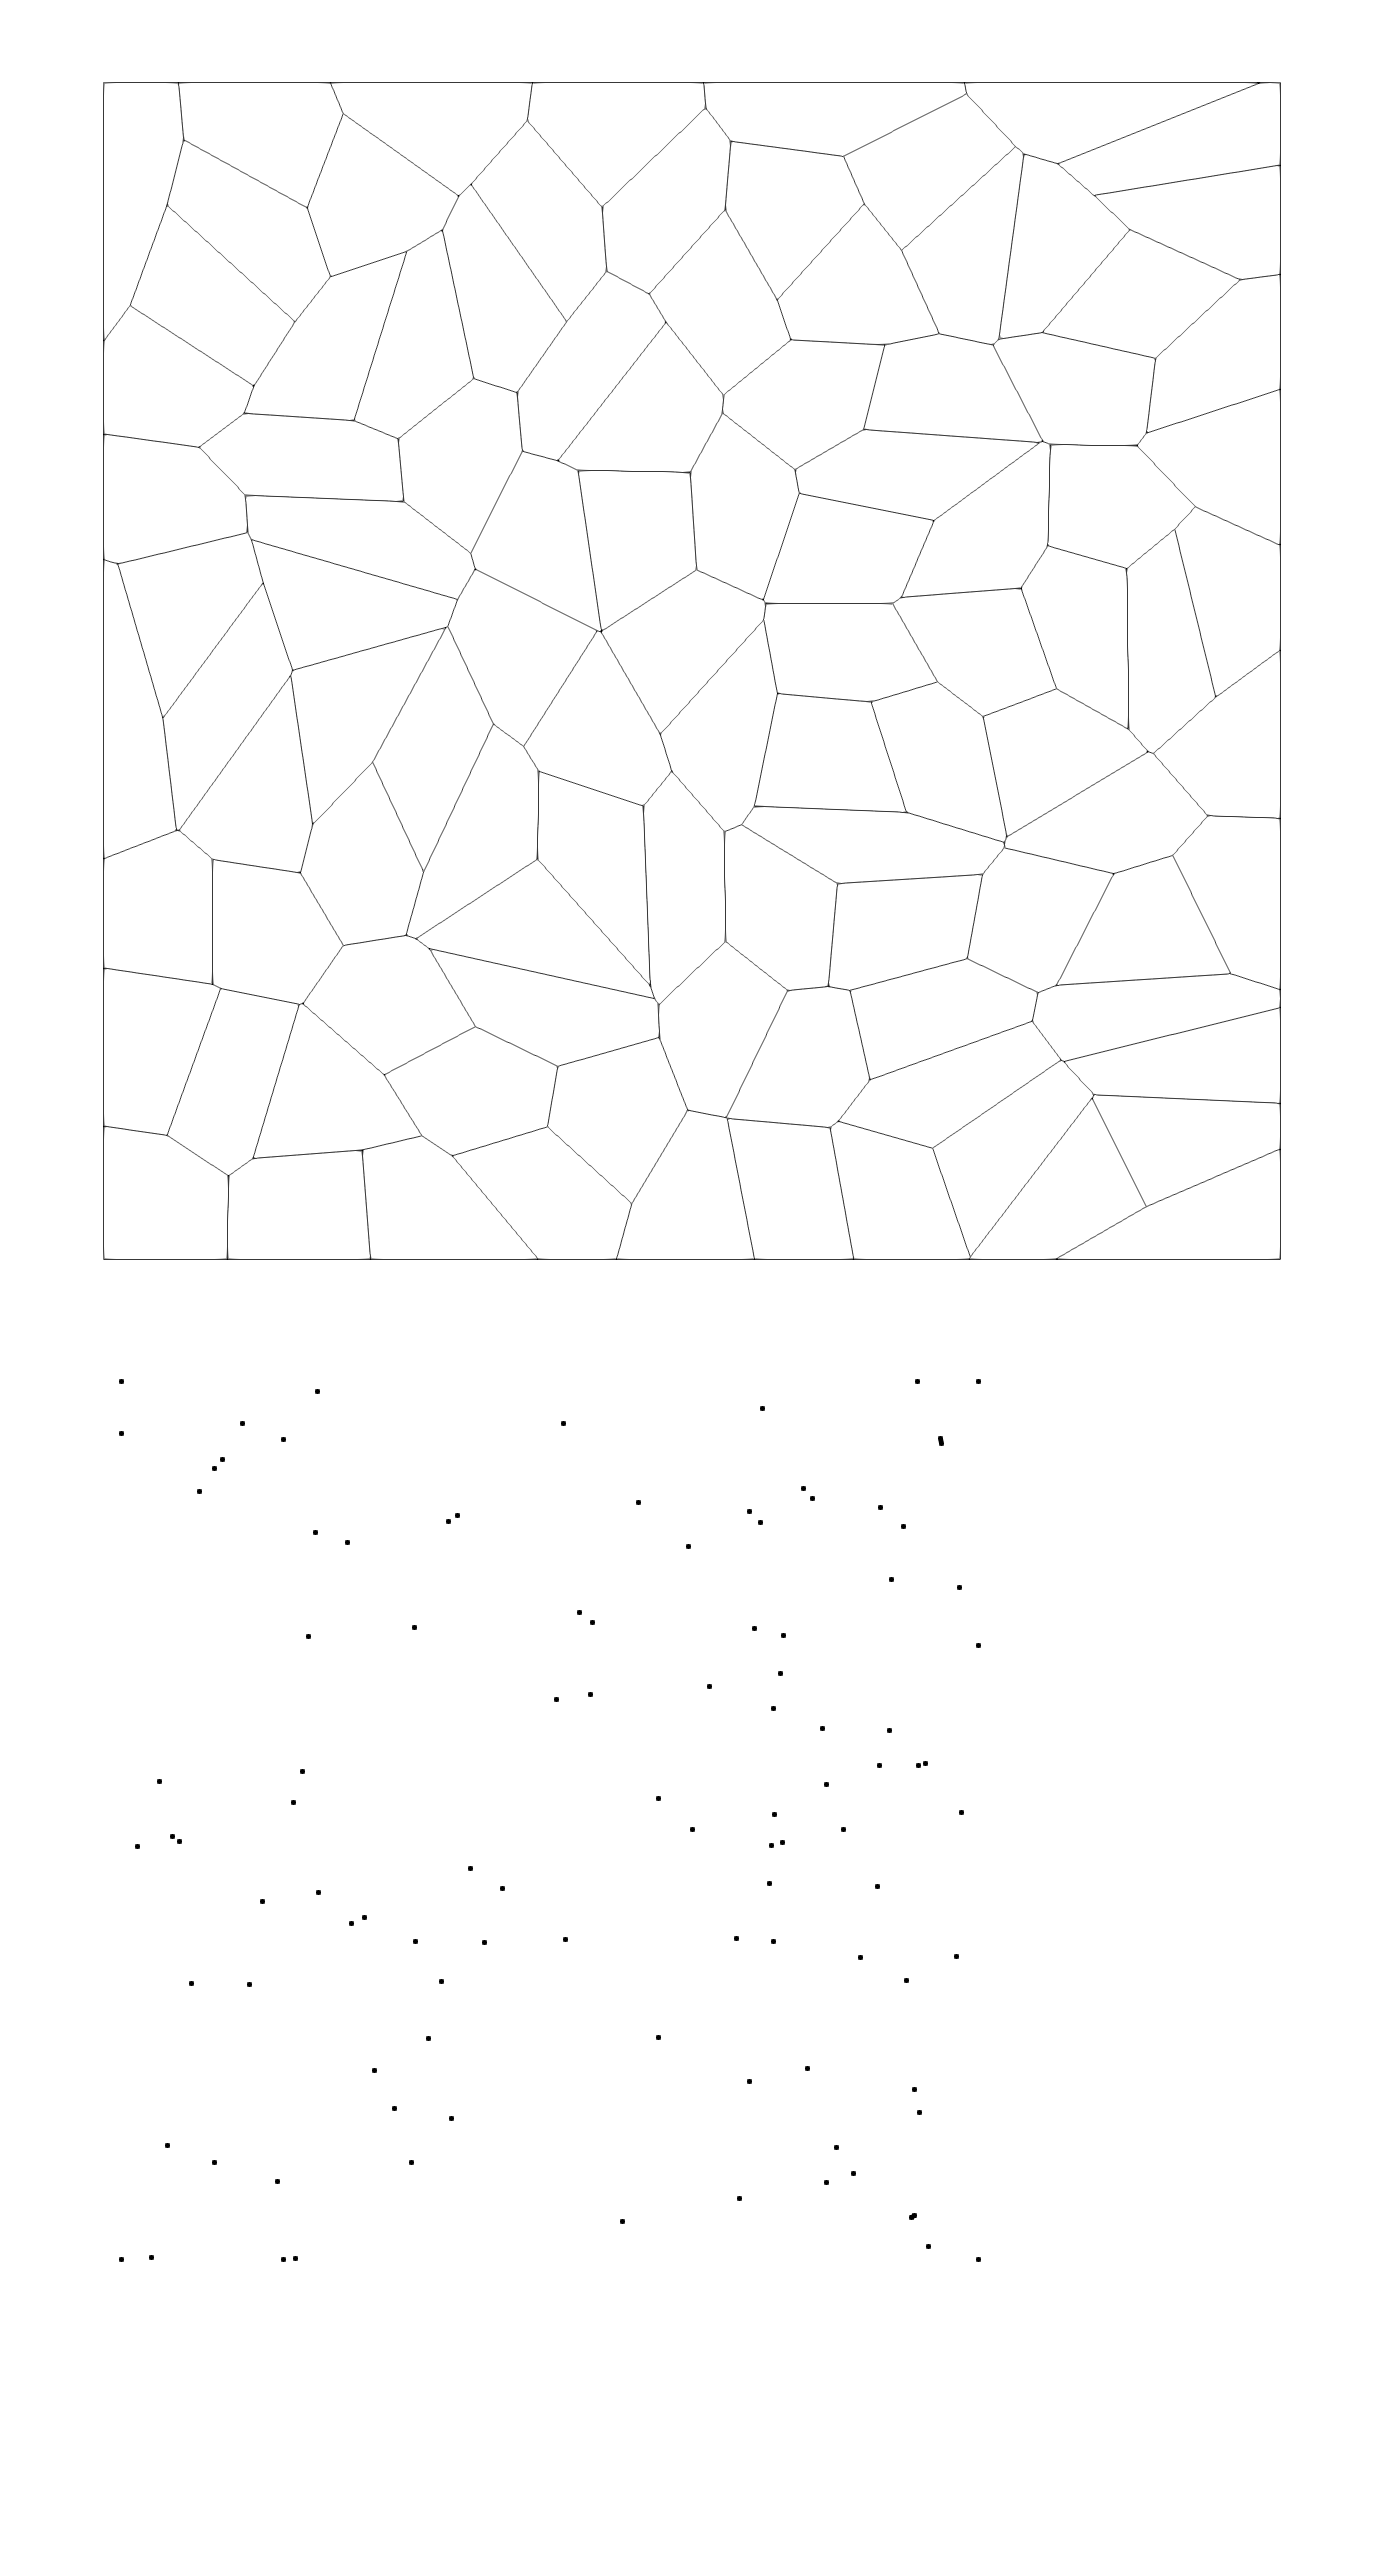
\includegraphics[height=0.8\textheight]{img/pd.png}
        \end{center}
    \end{minipage}
\end{frame}

\begin{frame}
    \frametitle{The world needs efficient power diagram computations !}

    Lot of work done before (Geogram, CGAL, ...), with a focus on the generic case.
    
    \vfill
    Most of the libraries are designed to give an \textit{exact connectivity}
    \begin{itemize}
        \item extra CPU and memory cost (bookkeeping)
        \item essentially sequential
    \end{itemize}

    \vfill
    SDOT application being more relaxed (need for simple integrals)
    \begin{itemize}
        \item development and test opportunities 
        \item scalability
    \end{itemize}
\end{frame}

\begin{frame}
    \frametitle{Individual cell computation}

    For each dirac $i$:
    \begin{itemize}
        \item starting from a non void finite cell (typically the domain boundaries),
        \item try some cuts with some \textit{close} diracs $j$
            \hfill{\textcolor{gray}{$\rightarrow$ Cell cuts}}

        \item until not possible to modify the cell
            \hfill{\textcolor{gray}{$\rightarrow$ Acceleration structures}}
    \end{itemize}
    
    \vfill
    Choices:
    \begin{itemize}
        \item infinite cells are handled by exceptions,
        \item tolerance on connectivity discrepancies (if zero mass),
        \item the sets of $j$ to test for a given $i$ are dynamic (dep. on updated cell geometry)
    \end{itemize}
    
\end{frame}

% ---------------------------------------------------------------------------------------
\section{Cell cuts}

\begin{frame}
    \frametitle{Test cases}

    Random distributions
    \begin{itemize}
        \item uniform in $[0,1]^{dim}$,
        \item uniform in the faces of a 20 points Voronoï diagram.
    \end{itemize}

    \vfill
    \begin{center}
        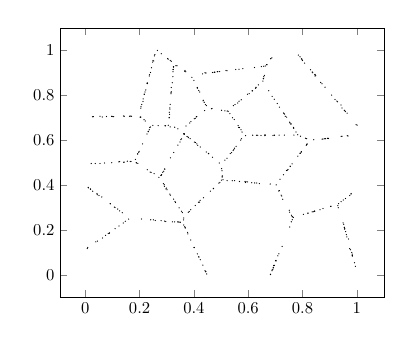
\begin{tikzpicture}[thick, scale=0.6]
  \begin{axis}
    \addplot [only marks, mark size=0.1pt] coordinates {
            ( 0.401544, 0.123371 )
            ( 0.377853, 0.18345 )
            ( 0.412696, 0.094736 )
            ( 0.367908, 0.211235 )
            ( 0.423769, 0.0686648 )
            ( 0.418974, 0.081198 )
            ( 0.376817, 0.190143 )
            ( 0.366483, 0.215511 )
            ( 0.444386, 0.0172317 )
            ( 0.362815, 0.222822 )
            ( 0.400546, 0.122734 )
            ( 0.440866, 0.0201061 )
            ( 0.433128, 0.0450913 )
            ( 0.388726, 0.156438 )
            ( 0.367847, 0.20972 )
            ( 0.417432, 0.0816121 )
            ( 0.44251, 0.0156105 )
            ( 0.447119, 0.00576412 )
            ( 0.0747329, 0.177071 )
            ( 0.00919154, 0.122965 )
            ( 0.0387603, 0.148201 )
            ( 0.159866, 0.249311 )
            ( 0.14745, 0.239462 )
            ( 0.139742, 0.231898 )
            ( 0.0449542, 0.15146 )
            ( 0.088092, 0.186434 )
            ( 0.0637233, 0.165528 )
            ( 0.12444, 0.218634 )
            ( 0.084978, 0.185211 )
            ( 0.10967, 0.206901 )
            ( 0.089022, 0.188134 )
            ( 0.00741753, 0.119004 )
            ( 0.0920801, 0.317235 )
            ( 0.0109817, 0.390008 )
            ( 0.011299, 0.387981 )
            ( 0.0439673, 0.357671 )
            ( 0.119323, 0.293905 )
            ( 0.0429018, 0.362898 )
            ( 0.061001, 0.347573 )
            ( 0.107255, 0.302591 )
            ( 0.0507313, 0.35375 )
            ( 0.13632, 0.277057 )
            ( 0.0918397, 0.317177 )
            ( 0.0190755, 0.381758 )
            ( 0.02746, 0.373235 )
            ( 0.109449, 0.300572 )
            ( 0.126635, 0.285666 )
            ( 0.0188767, 0.382924 )
            ( 0.362099, 0.245564 )
            ( 0.36272, 0.254164 )
            ( 0.349651, 0.235634 )
            ( 0.279251, 0.242196 )
            ( 0.292342, 0.240389 )
            ( 0.32916, 0.236807 )
            ( 0.250719, 0.24608 )
            ( 0.343366, 0.236085 )
            ( 0.240853, 0.246214 )
            ( 0.320898, 0.237004 )
            ( 0.29659, 0.238665 )
            ( 0.340185, 0.236596 )
            ( 0.25786, 0.243102 )
            ( 0.207233, 0.249925 )
            ( 0.348557, 0.235713 )
            ( 0.35744, 0.278164 )
            ( 0.287881, 0.406506 )
            ( 0.354158, 0.284218 )
            ( 0.332568, 0.322702 )
            ( 0.311538, 0.360218 )
            ( 0.330229, 0.327489 )
            ( 0.297141, 0.383311 )
            ( 0.345602, 0.299356 )
            ( 0.300887, 0.379342 )
            ( 0.313432, 0.355577 )
            ( 0.291518, 0.394532 )
            ( 0.290844, 0.401247 )
            ( 0.299599, 0.387113 )
            ( 0.325764, 0.337863 )
            ( 0.42289, 0.332439 )
            ( 0.388402, 0.290663 )
            ( 0.492044, 0.409178 )
            ( 0.379301, 0.279277 )
            ( 0.382741, 0.282647 )
            ( 0.435763, 0.344096 )
            ( 0.472659, 0.38579 )
            ( 0.501518, 0.422154 )
            ( 0.495689, 0.412113 )
            ( 0.46072, 0.37334 )
            ( 0.421067, 0.324555 )
            ( 0.471457, 0.383995 )
            ( 0.417274, 0.324305 )
            ( 0.405371, 0.309603 )
            ( 0.503962, 0.440295 )
            ( 0.503385, 0.46368 )
            ( 0.505547, 0.440522 )
            ( 0.504261, 0.435741 )
            ( 0.502188, 0.473228 )
            ( 0.235847, 0.645725 )
            ( 0.193568, 0.538155 )
            ( 0.231776, 0.639126 )
            ( 0.196664, 0.546065 )
            ( 0.237682, 0.65555 )
            ( 0.184627, 0.5142 )
            ( 0.240223, 0.658367 )
            ( 0.210942, 0.583013 )
            ( 0.231763, 0.637207 )
            ( 0.227269, 0.627243 )
            ( 0.192618, 0.53873 )
            ( 0.198327, 0.549974 )
            ( 0.242425, 0.456447 )
            ( 0.271217, 0.434741 )
            ( 0.239194, 0.457762 )
            ( 0.253525, 0.451026 )
            ( 0.188026, 0.498734 )
            ( 0.193552, 0.496707 )
            ( 0.228527, 0.468356 )
            ( 0.187737, 0.4998 )
            ( 0.281496, 0.446573 )
            ( 0.291954, 0.471644 )
            ( 0.313679, 0.521167 )
            ( 0.349106, 0.591581 )
            ( 0.325982, 0.544939 )
            ( 0.341471, 0.577581 )
            ( 0.278572, 0.443352 )
            ( 0.288869, 0.461714 )
            ( 0.363489, 0.627181 )
            ( 0.293188, 0.471166 )
            ( 0.354823, 0.605488 )
            ( 0.285621, 0.45732 )
            ( 0.364547, 0.626115 )
            ( 0.279549, 0.443197 )
            ( 0.352117, 0.601533 )
            ( 0.36294, 0.62782 )
            ( 0.364868, 0.627743 )
            ( 0.248791, 0.665193 )
            ( 0.268455, 0.663879 )
            ( 0.293726, 0.663089 )
            ( 0.295422, 0.66366 )
            ( 0.62384, 0.409627 )
            ( 0.522344, 0.419944 )
            ( 0.541253, 0.419339 )
            ( 0.631597, 0.409293 )
            ( 0.59233, 0.414986 )
            ( 0.589811, 0.411817 )
            ( 0.613001, 0.41051 )
            ( 0.567932, 0.416589 )
            ( 0.681065, 0.404703 )
            ( 0.597772, 0.414207 )
            ( 0.549887, 0.419916 )
            ( 0.641179, 0.407025 )
            ( 0.507048, 0.424134 )
            ( 0.588056, 0.416268 )
            ( 0.691789, 0.0328619 )
            ( 0.700765, 0.0650213 )
            ( 0.71307, 0.0952699 )
            ( 0.762318, 0.246425 )
            ( 0.702476, 0.0633627 )
            ( 0.693794, 0.0426857 )
            ( 0.687825, 0.0197334 )
            ( 0.693178, 0.0331661 )
            ( 0.694357, 0.0433754 )
            ( 0.682195, 0.00457597 )
            ( 0.702065, 0.0654758 )
            ( 0.688265, 0.023803 )
            ( 0.682097, 0.00291638 )
            ( 0.709139, 0.0862151 )
            ( 0.724989, 0.128042 )
            ( 0.752709, 0.214141 )
            ( 0.696754, 0.0438726 )
            ( 0.690764, 0.0260008 )
            ( 0.758737, 0.237057 )
            ( 0.954026, 0.21265 )
            ( 0.983216, 0.0937607 )
            ( 0.955186, 0.204367 )
            ( 0.983166, 0.0874571 )
            ( 0.952153, 0.226447 )
            ( 0.977038, 0.113283 )
            ( 0.973758, 0.11808 )
            ( 0.983633, 0.0885676 )
            ( 0.99487, 0.0394979 )
            ( 0.955631, 0.207233 )
            ( 0.983548, 0.0849575 )
            ( 0.954164, 0.2122 )
            ( 0.963397, 0.169964 )
            ( 0.930089, 0.308852 )
            ( 0.981456, 0.100674 )
            ( 0.961578, 0.180311 )
            ( 0.949485, 0.232201 )
            ( 0.991519, 0.0558627 )
            ( 0.96926, 0.160972 )
            ( 0.959128, 0.193755 )
            ( 0.932, 0.299507 )
            ( 0.8394, 0.282164 )
            ( 0.820604, 0.27626 )
            ( 0.904837, 0.305981 )
            ( 0.835659, 0.281202 )
            ( 0.766157, 0.256789 )
            ( 0.820127, 0.27451 )
            ( 0.864252, 0.290873 )
            ( 0.903651, 0.305434 )
            ( 0.803357, 0.27037 )
            ( 0.875614, 0.295951 )
            ( 0.844159, 0.285112 )
            ( 0.844939, 0.283784 )
            ( 0.95015, 0.334219 )
            ( 0.979216, 0.362321 )
            ( 0.942026, 0.326721 )
            ( 0.974251, 0.353962 )
            ( 0.932835, 0.317789 )
            ( 0.958299, 0.340723 )
            ( 0.978315, 0.360559 )
            ( 0.884245, 0.606443 )
            ( 0.891557, 0.607704 )
            ( 0.942423, 0.616458 )
            ( 0.967625, 0.617838 )
            ( 0.895772, 0.606694 )
            ( 0.893906, 0.607724 )
            ( 0.875263, 0.60455 )
            ( 0.945237, 0.616763 )
            ( 0.872203, 0.604342 )
            ( 0.965179, 0.619194 )
            ( 0.841707, 0.601548 )
            ( 0.882373, 0.605821 )
            ( 0.746442, 0.469522 )
            ( 0.795586, 0.548738 )
            ( 0.761518, 0.494455 )
            ( 0.817778, 0.582594 )
            ( 0.795023, 0.546448 )
            ( 0.716998, 0.426331 )
            ( 0.74076, 0.464931 )
            ( 0.815279, 0.581391 )
            ( 0.81376, 0.577051 )
            ( 0.78282, 0.528539 )
            ( 0.75481, 0.484307 )
            ( 0.754957, 0.482656 )
            ( 0.744571, 0.46664 )
            ( 0.79207, 0.541661 )
            ( 0.729761, 0.446162 )
            ( 0.790933, 0.541149 )
            ( 0.721396, 0.355263 )
            ( 0.714664, 0.375457 )
            ( 0.762837, 0.259288 )
            ( 0.70329, 0.401117 )
            ( 0.752627, 0.279839 )
            ( 0.723582, 0.351962 )
            ( 0.712755, 0.374192 )
            ( 0.727187, 0.337015 )
            ( 0.76184, 0.260274 )
            ( 0.759779, 0.266281 )
            ( 0.75133, 0.288826 )
            ( 0.126631, 0.50427 )
            ( 0.0219588, 0.495596 )
            ( 0.1238, 0.503108 )
            ( 0.0707419, 0.498496 )
            ( 0.141742, 0.501595 )
            ( 0.168433, 0.504859 )
            ( 0.165371, 0.504858 )
            ( 0.154912, 0.50624 )
            ( 0.0367013, 0.495782 )
            ( 0.143057, 0.502117 )
            ( 0.0976184, 0.499602 )
            ( 0.0539518, 0.49599 )
            ( 0.202376, 0.702544 )
            ( 0.202425, 0.701607 )
            ( 0.204523, 0.701866 )
            ( 0.220787, 0.684711 )
            ( 0.216545, 0.690528 )
            ( 0.166139, 0.706622 )
            ( 0.143557, 0.706054 )
            ( 0.0267046, 0.703742 )
            ( 0.0995202, 0.704468 )
            ( 0.104638, 0.703874 )
            ( 0.0299945, 0.703735 )
            ( 0.0975065, 0.705239 )
            ( 0.140717, 0.707121 )
            ( 0.162793, 0.705764 )
            ( 0.0626189, 0.702819 )
            ( 0.0544615, 0.705466 )
            ( 0.170183, 0.705884 )
            ( 0.0783252, 0.704276 )
            ( 0.227442, 0.852155 )
            ( 0.252418, 0.951249 )
            ( 0.24355, 0.921 )
            ( 0.207811, 0.758045 )
            ( 0.212675, 0.771565 )
            ( 0.228652, 0.853504 )
            ( 0.20471, 0.741552 )
            ( 0.205426, 0.747797 )
            ( 0.219948, 0.813662 )
            ( 0.217626, 0.802855 )
            ( 0.256353, 0.978895 )
            ( 0.254649, 0.973746 )
            ( 0.236782, 0.890044 )
            ( 0.24976, 0.953314 )
            ( 0.247804, 0.946085 )
            ( 0.229057, 0.850785 )
            ( 0.216839, 0.803914 )
            ( 0.222933, 0.822658 )
            ( 0.240582, 0.900001 )
            ( 0.235935, 0.884353 )
            ( 0.213182, 0.782587 )
            ( 0.386254, 0.606216 )
            ( 0.374975, 0.61593 )
            ( 0.380134, 0.610852 )
            ( 0.453465, 0.540458 )
            ( 0.414557, 0.577026 )
            ( 0.405887, 0.589332 )
            ( 0.410824, 0.583039 )
            ( 0.377717, 0.614408 )
            ( 0.423645, 0.569062 )
            ( 0.493682, 0.49805 )
            ( 0.445692, 0.547098 )
            ( 0.4018, 0.590995 )
            ( 0.454538, 0.539516 )
            ( 0.468774, 0.523924 )
            ( 0.544656, 0.553503 )
            ( 0.514234, 0.510915 )
            ( 0.575366, 0.606173 )
            ( 0.55531, 0.572009 )
            ( 0.547039, 0.557562 )
            ( 0.522118, 0.519393 )
            ( 0.549532, 0.56417 )
            ( 0.538893, 0.544293 )
            ( 0.572281, 0.599971 )
            ( 0.533745, 0.540201 )
            ( 0.573656, 0.645685 )
            ( 0.567938, 0.655333 )
            ( 0.542514, 0.698922 )
            ( 0.548485, 0.691241 )
            ( 0.526381, 0.727404 )
            ( 0.564607, 0.656253 )
            ( 0.532765, 0.717387 )
            ( 0.577354, 0.635459 )
            ( 0.56296, 0.664481 )
            ( 0.522715, 0.728719 )
            ( 0.465065, 0.738854 )
            ( 0.466651, 0.740319 )
            ( 0.501765, 0.731892 )
            ( 0.514244, 0.729992 )
            ( 0.308883, 0.698685 )
            ( 0.311658, 0.737725 )
            ( 0.325499, 0.924726 )
            ( 0.316839, 0.814053 )
            ( 0.305846, 0.665818 )
            ( 0.311451, 0.742814 )
            ( 0.322728, 0.881366 )
            ( 0.315622, 0.80586 )
            ( 0.309331, 0.700085 )
            ( 0.32328, 0.913849 )
            ( 0.323665, 0.913136 )
            ( 0.316736, 0.833013 )
            ( 0.320356, 0.854312 )
            ( 0.312889, 0.758499 )
            ( 0.310448, 0.714269 )
            ( 0.322935, 0.903516 )
            ( 0.32489, 0.924861 )
            ( 0.324802, 0.92475 )
            ( 0.315894, 0.81202 )
            ( 0.309572, 0.723667 )
            ( 0.341069, 0.650054 )
            ( 0.329154, 0.656995 )
            ( 0.312804, 0.658476 )
            ( 0.408963, 0.70419 )
            ( 0.409781, 0.704002 )
            ( 0.405166, 0.696902 )
            ( 0.410735, 0.703267 )
            ( 0.389204, 0.681986 )
            ( 0.385036, 0.675703 )
            ( 0.439578, 0.730936 )
            ( 0.401102, 0.694655 )
            ( 0.371161, 0.662609 )
            ( 0.412273, 0.831399 )
            ( 0.418011, 0.820279 )
            ( 0.412388, 0.833111 )
            ( 0.413483, 0.830923 )
            ( 0.434434, 0.776948 )
            ( 0.400167, 0.864723 )
            ( 0.446135, 0.753266 )
            ( 0.442439, 0.757483 )
            ( 0.392825, 0.878429 )
            ( 0.438169, 0.767359 )
            ( 0.42182, 0.81352 )
            ( 0.434139, 0.774113 )
            ( 0.337646, 0.929977 )
            ( 0.370215, 0.903588 )
            ( 0.367399, 0.908938 )
            ( 0.334111, 0.93035 )
            ( 0.366513, 0.905442 )
            ( 0.316725, 0.950053 )
            ( 0.305225, 0.959296 )
            ( 0.265804, 0.997924 )
            ( 0.279811, 0.982784 )
            ( 0.312973, 0.952887 )
            ( 0.303629, 0.961575 )
            ( 0.545468, 0.752474 )
            ( 0.615871, 0.81843 )
            ( 0.626773, 0.830187 )
            ( 0.628511, 0.834345 )
            ( 0.574442, 0.778481 )
            ( 0.637292, 0.845044 )
            ( 0.566513, 0.772484 )
            ( 0.551851, 0.757924 )
            ( 0.561549, 0.764178 )
            ( 0.628657, 0.832027 )
            ( 0.603578, 0.806105 )
            ( 0.614241, 0.818424 )
            ( 0.597666, 0.8033 )
            ( 0.630783, 0.621532 )
            ( 0.662671, 0.620973 )
            ( 0.691359, 0.6204 )
            ( 0.616435, 0.621463 )
            ( 0.695789, 0.621796 )
            ( 0.59023, 0.619744 )
            ( 0.661781, 0.623277 )
            ( 0.661416, 0.619688 )
            ( 0.647125, 0.620088 )
            ( 0.73325, 0.622112 )
            ( 0.635492, 0.621559 )
            ( 0.713772, 0.621907 )
            ( 0.69711, 0.621246 )
            ( 0.768475, 0.622224 )
            ( 0.475844, 0.901153 )
            ( 0.441347, 0.898753 )
            ( 0.474668, 0.900709 )
            ( 0.580411, 0.91679 )
            ( 0.486228, 0.903614 )
            ( 0.663074, 0.928631 )
            ( 0.518028, 0.908771 )
            ( 0.432092, 0.893721 )
            ( 0.495052, 0.904009 )
            ( 0.48811, 0.903767 )
            ( 0.522303, 0.907705 )
            ( 0.554461, 0.913063 )
            ( 0.566033, 0.914361 )
            ( 0.468595, 0.899643 )
            ( 0.444289, 0.897653 )
            ( 0.477469, 0.901822 )
            ( 0.623031, 0.922159 )
            ( 0.657232, 0.927515 )
            ( 0.648618, 0.926383 )
            ( 0.815331, 0.606214 )
            ( 0.792884, 0.61728 )
            ( 0.811107, 0.608383 )
            ( 0.837871, 0.8985 )
            ( 0.867214, 0.856023 )
            ( 1.00109, 0.666276 )
            ( 0.997418, 0.668451 )
            ( 0.928938, 0.770271 )
            ( 0.942013, 0.755757 )
            ( 0.846155, 0.884908 )
            ( 0.800111, 0.953515 )
            ( 0.95811, 0.726328 )
            ( 0.919799, 0.780482 )
            ( 0.845512, 0.890326 )
            ( 0.797122, 0.959784 )
            ( 0.848916, 0.885641 )
            ( 0.926817, 0.773009 )
            ( 0.796013, 0.960777 )
            ( 0.955369, 0.73028 )
            ( 0.964298, 0.719443 )
            ( 0.883279, 0.834579 )
            ( 0.807908, 0.941779 )
            ( 0.846394, 0.891378 )
            ( 0.790886, 0.969376 )
            ( 0.953755, 0.732249 )
            ( 0.907572, 0.799682 )
            ( 0.835753, 0.901824 )
            ( 0.798526, 0.956175 )
            ( 0.872049, 0.849825 )
            ( 0.82955, 0.912344 )
            ( 0.784679, 0.977251 )
            ( 0.945447, 0.742717 )
            ( 0.669659, 0.934312 )
            ( 0.683195, 0.960629 )
            ( 0.667696, 0.934703 )
            ( 0.687384, 0.964955 )
            ( 0.683461, 0.961691 )
            ( 0.654253, 0.861951 )
            ( 0.656709, 0.872887 )
            ( 0.655522, 0.872552 )
            ( 0.659996, 0.887117 )
            ( 0.657666, 0.880946 )
            ( 0.782583, 0.623616 )
            ( 0.776121, 0.63569 )
            ( 0.696013, 0.781282 )
            ( 0.767663, 0.6523 )
            ( 0.730099, 0.72007 )
            ( 0.736858, 0.705758 )
            ( 0.752703, 0.679175 )
            ( 0.754055, 0.675783 )
            ( 0.757818, 0.67207 )
            ( 0.688233, 0.793702 )
            ( 0.731753, 0.717696 )
            ( 0.714923, 0.745965 )
            ( 0.67594, 0.818907 )
            ( 0.757304, 0.670805 )
            ( 0.767296, 0.656222 )
            ( 0.766483, 0.653808 )
            ( 0.741683, 0.70206 )
            ( 0.707121, 0.762002 )
            ( 0.733877, 0.715258 )
    };
  \end{axis}
\end{tikzpicture}

        \kern 1cm
        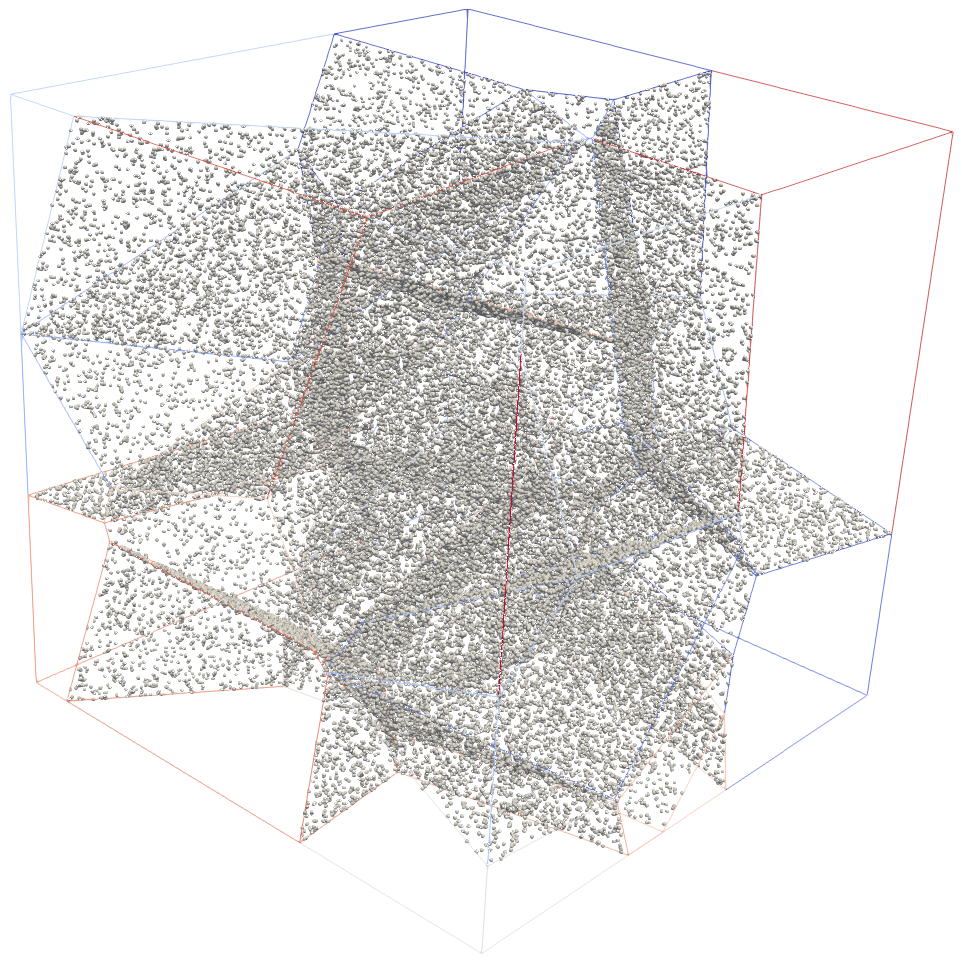
\includegraphics[width=0.26\textwidth]{img/voro_distrib_3d.png}
    \end{center}
\end{frame}

\begin{frame}
    \frametitle{Distribution of $\#$ nodes per cell before each cut, 2D case}

    \begin{minipage}[c][0.6\textheight][c]{0.4\textwidth}
        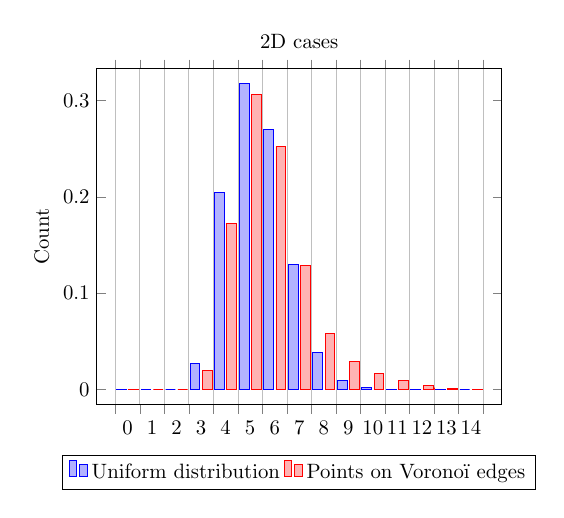
\begin{tikzpicture}[scale=0.75]
    \begin{axis}[
        legend style={at={(0.5,-0.15)},anchor=north,legend columns=-1},
        ybar interval=0.8,
        ylabel=Count,
        title=2D cases,
        enlargelimits=0.05,
    ]
    \addplot coordinates {
       ( 0, 1.58049e-06 )           
       ( 1, 0           )
       ( 2, 0           )
       ( 3, 0.0269854   )         
       ( 4, 0.204727    )        
       ( 5, 0.317403    )        
       ( 6, 0.270196    )        
       ( 7, 0.129706    )        
       ( 8, 0.0389355   )         
       ( 9, 0.00941079  )          
       (10, 0.00214473  )          
       (11, 0.000444119 )           
       (12, 4.47807e-05 )
       (13, 2.10733e-06 )
       (14, 0           )
       (15, 0           )
       % (16, 0           )
       % (17, 0           )
       % (18, 0           )
       % (19, 0           )
    };
    \addplot coordinates {
       ( 0, 7.68332e-06 )
       ( 1, 0           )
       ( 2, 0           )
       ( 3, 0.0202567   )
       ( 4, 0.172274    )
       ( 5, 0.306317    )
       ( 6, 0.252301    )
       ( 7, 0.128378    )
       ( 8, 0.0579965   )
       ( 9, 0.028838    )
       (10, 0.0167608   )
       (11, 0.00910499  )
       (12, 0.00417465  )
       (13, 0.00208543  )
       (13, 0.000886446 )
       (14, 0.00030603  )
       (15, 0.000186223 )
       % (16, 8.26933e-05 )
       % (17, 3.29471e-05 )
       % (18, 7.55309e-06 )
       % (19, 3.51609e-06 )
    };
    \legend{Uniform distribution,Points on Voronoï edges}
    \end{axis}
\end{tikzpicture}

    \end{minipage}
    \kern 0.04\textwidth
    \begin{minipage}{0.55\textwidth}
        \begin{itemize}
            \item Before the cuts, most of the cells have less than 8 nodes
            
            \bigskip
            \item With SIMD instructions, testing all the nodes at once will
                  always be faster than selective testing. 
                  \\ \hfill {\textcolor{gray}{$\Rightarrow$ \texttt{\_mm512\_cmp\_pd\_mask} or similar}}
                  \\ \hfill {\textcolor{gray}{with a struct of aligned blocks}}
              \end{itemize}
    \end{minipage}
\end{frame}

\begin{frame}
    \frametitle{Distribution of $\#$ outside nodes during each cut, 2D case}

    \begin{minipage}[c][0.6\textheight][c]{0.4\textwidth}
        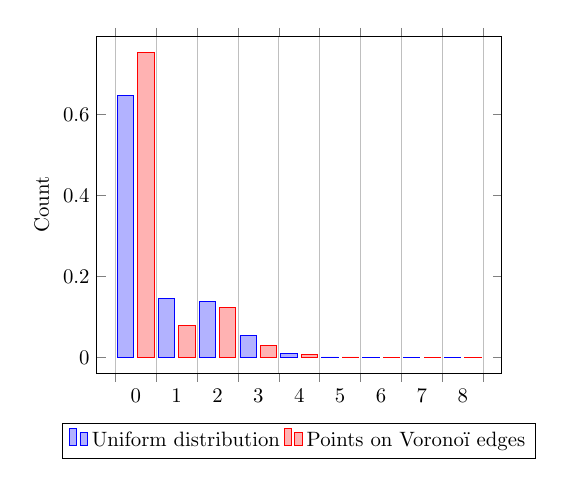
\begin{tikzpicture}[scale=0.75]
    \begin{axis}[
        legend style={at={(0.5,-0.15)},anchor=north,legend columns=-1},
        ybar interval=0.8,
        ylabel=Count,
        enlargelimits=0.05,
    ]
    \addplot coordinates {
       ( 0, 0.646137    )           
       ( 1, 0.145905    )
       ( 2, 0.139458    )
       ( 3, 0.054996    )         
       ( 4, 0.0113526   )        
       ( 5, 0.00182122  )        
       ( 6, 0.000274437 )        
       ( 7, 3.82628e-05 )        
       ( 8, 1.71523e-05 )         
       ( 9, 8.79605e-07 )
    };
    \addplot coordinates {
       ( 0, 0.754382    )           
       ( 1, 0.080362    )
       ( 2, 0.124597    )
       ( 3, 0.0302812   )         
       ( 4, 0.00826525  )        
       ( 5, 0.00181659  )        
       ( 6, 0.000260039 )        
       ( 7, 3.39893e-05 )        
       ( 8, 1.43329e-06 )         
       ( 9, 2.04755e-07 )
    };
    \legend{Uniform distribution,Points on Voronoï edges}
    \end{axis}
\end{tikzpicture}

    \end{minipage}
    \kern 0.04\textwidth
    \begin{minipage}{0.55\textwidth}
        \begin{itemize}
            \item Need for quick eviction of the no-cut case.
            
            \bigskip
            \item The number of node in / node out combinations will be reasonably limited. 
            \\ \hfill {\textcolor{gray}{$\Rightarrow$ code generation !}}
        \end{itemize}
    \end{minipage}
\end{frame}


\begin{frame}[fragile]
    \frametitle{Code generation for the 2D case}

    Offline optimization (for the vector of booleans, true if outside):
    \begin{itemize}
        \item all the relevant information stay in registers 
              (minimization of load and stores)
        \item minimization of moves (cyclicity) and scalar operations
    \end{itemize}

\begin{footnotesize}
\begin{lstlisting} 
case 1017: { // size=3 outside=...00000000000001 mod=[ 0, 1 ],1,2,[ 0, 2 ]
    size = 4; // we're adding a new node (staying with the same registers)
    ... // a constant to select between original node vs interpolated ones
    __m512i id_0 = _mm512_cvtepu8_epi64( _mm_cvtsi64_si128( 0x9020108ul ) );
    ... // interpolations
    __m128d x_i0 = _mm_set1_pd( x_0 );     // SSE2 is enough to compute 
    __m128d x_i1 = _mm_set_pd( x_2, x_1 ); // them
    __m128d m = _mm_div_pd( d_i0, _mm_sub_pd( d_i1, d_i0 ) );
    __m512d inter_x = _mm512_castpd128_pd512( 
        _mm_sub_pd( x_i0, _mm_mul_pd( m, _mm_sub_pd( x_i1, x_i0 ) ) )
    );
    ... // store within the same registers
    px_0 = _mm512_permutex2var_pd( px_0, id_0, inter_x );
    break;
}
\end{lstlisting}
\end{footnotesize}
\end{frame}

\begin{frame}
    \frametitle{Speedup due to code generation}

    Time per effective cut:

    \medskip
    \begin{center}    
    \begin{tabular}{|l|c|c|}
        \hline
        Method                 & CPU cycles & Speedup    \\
        \hline
        Optimized generic code & 80         & 1.0 $\times$ \\
        Optimized AVX512 code  & 50         & 1.6 $\times$ \\
        Generated AVX512 code  & 23         & 3.5 $\times$ \\
        \hline
    \end{tabular}
    \end{center}
\end{frame}


\begin{frame}
    \frametitle{Distribution of $\#$ nodes per cell before each cut, 3D case}

    \begin{minipage}[c][0.6\textheight][c]{0.4\textwidth}
        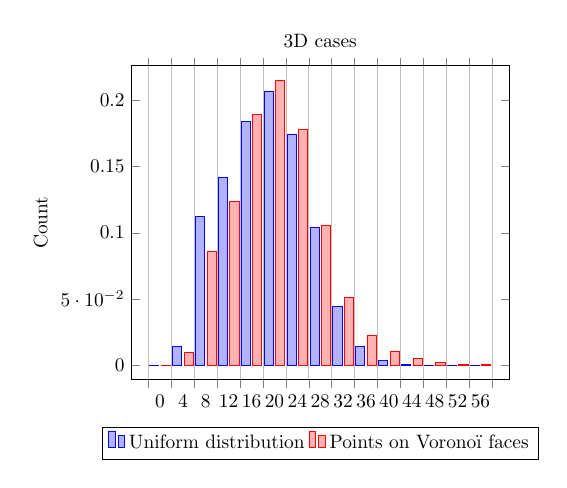
\begin{tikzpicture}[scale=0.7]
    \begin{axis}[
        legend style={at={(0.5,-0.15)},anchor=north,legend columns=-1},
        ybar interval=0.8,
        ylabel=Count,
        title=3D cases,
        enlargelimits=0.05,
    ]
    \addplot coordinates {
        (  0, 8.486250e-07 )
        (  4, 1.407526e-02 )
        (  8, 1.121475e-01 )
        ( 12, 1.418800e-01 )
        ( 16, 1.838793e-01 )
        ( 20, 2.061940e-01 )
        ( 24, 1.739535e-01 )
        ( 28, 1.041492e-01 )
        ( 32, 4.463720e-02 )
        ( 36, 1.415705e-02 )
        ( 40, 3.759130e-03 )
        ( 44, 8.953000e-04 )
        ( 48, 2.305428e-04 )
        ( 52, 2.970185e-05 )
        ( 56, 5.657500e-06 )
        ( 60, 1.697250e-06 )
        %(  0, 8.48625e-07 )
        %(  2, 0           )
        %(  4, 0.00166076  )
        %(  6, 0.0124145   )
        %(  8, 0.055026    )
        %( 10, 0.0571215   )
        %( 12, 0.0658276   )
        %( 14, 0.0760524   )
        %( 16, 0.0868673   )
        %( 18, 0.097012    )
        %( 20, 0.102684    )
        %( 22, 0.10351     )
        %( 24, 0.0937935   )
        %( 26, 0.08016     )
        %( 28, 0.0611126   )
        %( 30, 0.0430366   )
        %( 32, 0.027646    )
        %( 34, 0.0169912   )
        %( 36, 0.00930461  )
        %( 38, 0.00485244  )
        %( 40, 0.00249666  )
        %( 42, 0.00126247  )
        %( 44, 0.000582723 )
        %( 46, 0.000312577 )
        %( 48, 0.00016435  )
        %( 50, 6.61928e-05 )
        %( 52, 2.00841e-05 )
        %( 54, 9.61775e-06 )
        %( 56, 2.82875e-06 )
        %( 58, 2.82875e-06 )
        %( 60, 8.48625e-07 )
        %( 62, 8.48625e-07 )
        %( 64, 4.526e-06   )
    };
    \addplot coordinates {
        (  0, 1.505050e-06 )
        (  4, 9.766150e-03 )
        (  8, 8.581940e-02 )
        ( 12, 1.237691e-01 )
        ( 16, 1.892904e-01 )
        ( 20, 2.150680e-01 )
        ( 24, 1.776119e-01 )
        ( 28, 1.058479e-01 )
        ( 32, 5.102420e-02 )
        ( 36, 2.251171e-02 )
        ( 40, 1.034158e-02 )
        ( 44, 4.915620e-03 )
        ( 48, 2.280648e-03 )
        ( 52, 1.025441e-03 )
        ( 56, 4.561560e-04 )
        ( 60, 1.724536e-04 )
        % ( 64, 5.869700e-05 )
        % ( 68, 2.433162e-05 )
        % ( 72, 1.028451e-05 )
        % ( 76, 3.135520e-06 )
    };
    \legend{Uniform distribution,Points on Voronoï faces}
    \end{axis}
\end{tikzpicture}

    \end{minipage}
    \kern 0.04\textwidth
    \begin{minipage}{0.55\textwidth}
        \begin{itemize}
            \item Most of the cells have less than 32 nodes.
            
            \bigskip
            \item SIMD might be still competitive (maybe better to evaluate all at once than test which one
            to evaluate)
                \\ \hfill {\textcolor{gray}{$\Rightarrow$ struct of aligned blocks}}
        \end{itemize}
    \end{minipage}
\end{frame}

\begin{frame}
    \frametitle{Distribution of $\#$ outside nodes during each cut, 3D case}

    \begin{minipage}[c][0.6\textheight][c]{0.4\textwidth}
        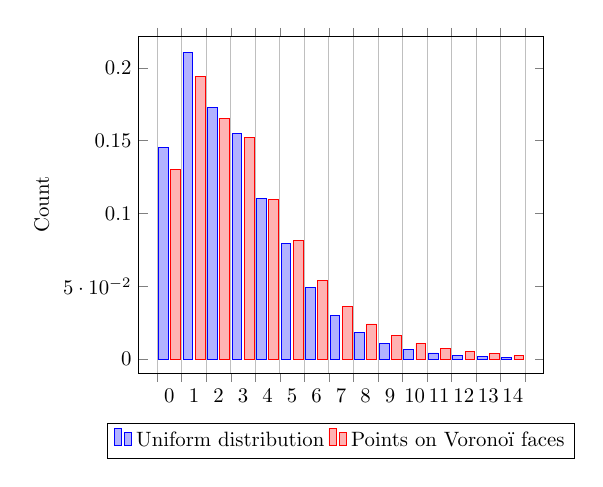
\begin{tikzpicture}[scale=0.75]
    \begin{axis}[
        legend style={at={(0.5,-0.15)},anchor=north,legend columns=-1},
        ybar interval=0.8,
        ylabel=Count,
        enlargelimits=0.05,
    ]
    \addplot coordinates {
        (  0, 0.145435    )
        (  1, 0.210804    )
        (  2, 0.172496    )
        (  3, 0.15462     )
        (  4, 0.110417    )
        (  5, 0.0792335   )
        (  6, 0.0491028   )
        (  7, 0.029678    )
        (  8, 0.018182    )
        (  9, 0.0107639   )
        ( 10, 0.0066061   )
        ( 11, 0.0041224   )
        ( 12, 0.00258985  )
        ( 13, 0.00182967  )
        ( 14, 0.00115674  )
        ( 15, 0.00084376  )
        % ( 16, 0.000590571 )
        % ( 17, 0.000383749 )
        % ( 18, 0.000338602 )
        % ( 19, 0.000234276 )
        % ( 20, 0.000137881 )
        % ( 21, 0.000108597 )
        % ( 22, 7.8092e-05  )
        % ( 23, 6.467e-05   )
        % ( 24, 2.98946e-05 )
        % ( 25, 3.72157e-05 )
        % ( 26, 2.68441e-05 )
        % ( 27, 2.98946e-05 )
        % ( 28, 1.70826e-05 )
        % ( 29, 1.64725e-05 )
        % ( 30, 1.22019e-05 )
        % ( 31, 1.22019e-06 )
        % ( 32, 3.66056e-06 )
        % ( 33, 0           )
        % ( 34, 1.22019e-06 )
        % ( 35, 3.05047e-06 )
        % ( 36, 3.66056e-06 )
    };
    \addplot coordinates {
        (  0, 0.130065    )
        (  1, 0.194111    )
        (  2, 0.165037    )
        (  3, 0.151967    )
        (  4, 0.109601    )
        (  5, 0.0815736   )
        (  6, 0.0537573   )
        (  7, 0.0360191   )
        (  8, 0.0240276   )
        (  9, 0.0160771   )
        ( 10, 0.0109301   )
        ( 11, 0.00749046  )
        ( 12, 0.00527951  )
        ( 13, 0.0038034   )
        ( 14, 0.00268949  )
        ( 15, 0.00200559  )
        % ( 16, 0.00144206  )
        % ( 17, 0.00102518  )
        % ( 18, 0.00077371  )
        % ( 19, 0.00059677  )
        % ( 20, 0.000475593 )
        % ( 21, 0.000328143 )
        % ( 22, 0.000243426 )
        % ( 23, 0.000187127 )
        % ( 24, 0.000137263 )
        % ...
    };
    \legend{Uniform distribution,Points on Voronoï faces}
    \end{axis}
\end{tikzpicture}

    \end{minipage}
    \kern 0.04\textwidth
    \begin{minipage}{0.55\textwidth}
        \begin{itemize}
            \item Majority of small cuts

            \bigskip
            \item OK to test all the nodes (in/out), but not each face (rem/cut/in).

            \bigskip
            \item OK for a switch/case for each face with a cut but not for the whole cell.
        \end{itemize}
    \end{minipage}
\end{frame}

\begin{frame}[fragile]
    \frametitle{Structures for 3D cells, compact blocks (simplified)}

    \begin{footnotesize}
    \begin{lstlisting} 
struct NodeBlock {
    Scalar x            [ 64 ]; // struct of block (SIMD)
    Scalar y            [ 64 ]; // sizeof( Scalar ) == sizeof( Edge )
    Scalar z            [ 64 ]; // sizeof( Scalar ) == sizeof( Face * )
    Edge   next_in_faces[ 64 ][ 3 ]; // exactly 3 edges per node 
    Edge   sibling_edges[ 64 ][ 3 ]; // sames edges, in reverse order
    Face  *faces        [ 64 ][ 3 ]; // sizeof( double )
};
struct Edge {
    NodeBlock *nptr_with_offset; // pointer + int in { 0, 1, 2 }
};
struct Face {
    Edge   first_edge; // linked list
    uint64 num_cut;    // to known if already visited
};
struct Cell {
    Pool<Face> faces;  // to have pointer stability
    NodeBlock *nodes;  // aligned
    uint64     nb_cut; // compared to face->num_cut
};
    \end{lstlisting}
    \end{footnotesize}
\end{frame}

% \begin{frame}
%     \frametitle{Cut procedure, SIMD case}

%     \begin{itemize}
%         \item Batch eval of the distances node / plane
%         \item For each outside node, for each not yet traversed connected face
%         \item \ \kern 2mm Add/retrieve node for each in/out edge, assign to edge number 0/1
%         \item \ \kern 2mm Remove outside faces
%         \item Create a new face, edge number 2
%     \end{itemize}
% \end{frame}

\begin{frame}[fragile]
    \frametitle{Structures for 3D cells, pools and linked lists (simplified)}

\begin{footnotesize}
\begin{lstlisting} 
struct Face {
    Point  cut_O, cut_N;
    Dirac *cut_id;
    Edge  *edges;    
};
struct Node {
    Edge *edge; // first edge of the linked list
    Point pos;
};
struct Edge {
    Edge *next_from_same_node, *next_from_same_face, *sibling;
    Node *n0, *n1;  
    Face *face;
};

PoolAc<Face> faces; // Pool with a foreach
PoolAc<Hole> holes; // for sphere cuts
PoolAc<Node> nodes; // => outside node found using max(dot(.,N))
Pool  <Edge> edges; // no need for an "active" list 
\end{lstlisting}
\end{footnotesize}
\end{frame}

\begin{frame}
    \frametitle{Speedups}

    Time per effective cut:

    \medskip
    \begin{center}    
    \begin{tabular}{|l|c|c|}
        \hline
        Method                   & CPU cycles & Speedup    \\
        \hline
        Struct of compact blocks & 782        & 1.0 $\times$ \\
        Pools and linked lists   & 392        & 2.0 $\times$ \\
        \hline
    \end{tabular}
    \end{center}
\end{frame}

% ---------------------------------------------------------------------------------------
\section{Acceleration structures}

\begin{frame}
    \frametitle{Algorithmic complexity}

    $\forall\ i, j \neq i $ basically gives $ \mathcal{O}( n^2 )$... would be far behind the 
      expected $\mathcal{O}( n \log{}n )$
    
    \vfill
    But only a small neighborhood is actually needed !

    \vfill
    Given radius around each dirac works very well for isotropic cells.
    
    \vfill
    New algorithms remained to be tested for the \textbf{anisotropic or not regular} cases.
\end{frame}

\begin{frame}
    \frametitle{If homogeneous Kantorovich potentials}

    \begin{minipage}[c][0.6\textheight][c]{0.6\textwidth}
        Algorithm:
        \begin{itemize}
            \item From a large enough cell ($\supset$ domain if finite),
            \item cut with the \textit{closest} diracs,
            \item until no longer possible to shrink the cell \\ \hfill \textcolor{gray}{($\Rightarrow$ dynamic criterion)}
        \end{itemize}

        \vfill
        Use of Lebesgue space filling curve (zgrids):
        \begin{itemize}
            \item $\mathcal{O}( n )$ pass to sort the nodes ($\parallelsum$ radix sort)
            \item $\mathcal{O}( n )$ pass to construct the grid
            \item $\mathcal{O}( n )$ pass to get the neighbors ($\parallelsum$ radix sort)
        \end{itemize}
    \end{minipage}
    \kern 0.04\textwidth
    \begin{minipage}{0.35\textwidth}
        \begin{center}
            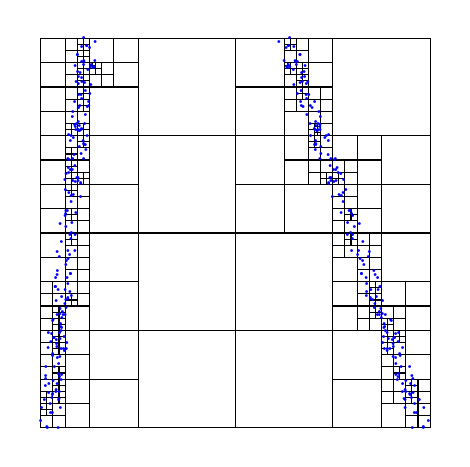
\begin{tikzpicture}[scale=0.5]

\draw (0.0521087,0.0323146) -- (0.36117,0.0323146) -- (0.36117,0.341376) -- (0.0521087,0.341376) -- (0.0521087,0.0323146) ;
\draw (0.36117,0.0323146) -- (0.670232,0.0323146) -- (0.670232,0.341376) -- (0.36117,0.341376) -- (0.36117,0.0323146) ;
\draw (0.0521087,0.341376) -- (0.206639,0.341376) -- (0.206639,0.495907) -- (0.0521087,0.495907) -- (0.0521087,0.341376) ;
\draw (0.206639,0.341376) -- (0.36117,0.341376) -- (0.36117,0.495907) -- (0.206639,0.495907) -- (0.206639,0.341376) ;
\draw (0.0521087,0.495907) -- (0.206639,0.495907) -- (0.206639,0.650438) -- (0.0521087,0.650438) -- (0.0521087,0.495907) ;
\draw (0.206639,0.495907) -- (0.36117,0.495907) -- (0.36117,0.650438) -- (0.206639,0.650438) -- (0.206639,0.495907) ;
\draw (0.36117,0.341376) -- (0.670232,0.341376) -- (0.670232,0.650438) -- (0.36117,0.650438) -- (0.36117,0.341376) ;
\draw (0.670232,0.0323146) -- (1.28835,0.0323146) -- (1.28835,0.650438) -- (0.670232,0.650438) -- (0.670232,0.0323146) ;
\draw (0.0521087,0.650438) -- (0.206639,0.650438) -- (0.206639,0.804969) -- (0.0521087,0.804969) -- (0.0521087,0.650438) ;
\draw (0.206639,0.650438) -- (0.36117,0.650438) -- (0.36117,0.804969) -- (0.206639,0.804969) -- (0.206639,0.650438) ;
\draw (0.0521087,0.804969) -- (0.206639,0.804969) -- (0.206639,0.959499) -- (0.0521087,0.959499) -- (0.0521087,0.804969) ;
\draw (0.206639,0.804969) -- (0.36117,0.804969) -- (0.36117,0.959499) -- (0.206639,0.959499) -- (0.206639,0.804969) ;
\draw (0.36117,0.650438) -- (0.515701,0.650438) -- (0.515701,0.804969) -- (0.36117,0.804969) -- (0.36117,0.650438) ;
\draw (0.515701,0.650438) -- (0.670232,0.650438) -- (0.670232,0.804969) -- (0.515701,0.804969) -- (0.515701,0.650438) ;
\draw (0.36117,0.804969) -- (0.515701,0.804969) -- (0.515701,0.959499) -- (0.36117,0.959499) -- (0.36117,0.804969) ;
\draw (0.515701,0.804969) -- (0.670232,0.804969) -- (0.670232,0.959499) -- (0.515701,0.959499) -- (0.515701,0.804969) ;
\draw (0.0521087,0.959499) -- (0.36117,0.959499) -- (0.36117,1.26856) -- (0.0521087,1.26856) -- (0.0521087,0.959499) ;
\draw (0.36117,0.959499) -- (0.515701,0.959499) -- (0.515701,1.11403) -- (0.36117,1.11403) -- (0.36117,0.959499) ;
\draw (0.515701,0.959499) -- (0.670232,0.959499) -- (0.670232,1.11403) -- (0.515701,1.11403) -- (0.515701,0.959499) ;
\draw (0.36117,1.11403) -- (0.515701,1.11403) -- (0.515701,1.26856) -- (0.36117,1.26856) -- (0.36117,1.11403) ;
\draw (0.515701,1.11403) -- (0.670232,1.11403) -- (0.670232,1.26856) -- (0.515701,1.26856) -- (0.515701,1.11403) ;
\draw (0.670232,0.650438) -- (1.28835,0.650438) -- (1.28835,1.26856) -- (0.670232,1.26856) -- (0.670232,0.650438) ;
\draw (1.28835,0.0323146) -- (2.5246,0.0323146) -- (2.5246,1.26856) -- (1.28835,1.26856) -- (1.28835,0.0323146) ;
\draw (0.0521087,1.26856) -- (0.36117,1.26856) -- (0.36117,1.57762) -- (0.0521087,1.57762) -- (0.0521087,1.26856) ;
\draw (0.36117,1.26856) -- (0.515701,1.26856) -- (0.515701,1.42309) -- (0.36117,1.42309) -- (0.36117,1.26856) ;
\draw (0.515701,1.26856) -- (0.670232,1.26856) -- (0.670232,1.42309) -- (0.515701,1.42309) -- (0.515701,1.26856) ;
\draw (0.36117,1.42309) -- (0.515701,1.42309) -- (0.515701,1.57762) -- (0.36117,1.57762) -- (0.36117,1.42309) ;
\draw (0.515701,1.42309) -- (0.670232,1.42309) -- (0.670232,1.57762) -- (0.515701,1.57762) -- (0.515701,1.42309) ;
\draw (0.0521087,1.57762) -- (0.36117,1.57762) -- (0.36117,1.88668) -- (0.0521087,1.88668) -- (0.0521087,1.57762) ;
\draw (0.36117,1.57762) -- (0.670232,1.57762) -- (0.670232,1.88668) -- (0.36117,1.88668) -- (0.36117,1.57762) ;
\draw (0.670232,1.26856) -- (1.28835,1.26856) -- (1.28835,1.88668) -- (0.670232,1.88668) -- (0.670232,1.26856) ;
\draw (0.0521087,1.88668) -- (0.36117,1.88668) -- (0.36117,2.19575) -- (0.0521087,2.19575) -- (0.0521087,1.88668) ;
\draw (0.36117,1.88668) -- (0.515701,1.88668) -- (0.515701,2.04121) -- (0.36117,2.04121) -- (0.36117,1.88668) ;
\draw (0.515701,1.88668) -- (0.670232,1.88668) -- (0.670232,2.04121) -- (0.515701,2.04121) -- (0.515701,1.88668) ;
\draw (0.36117,2.04121) -- (0.515701,2.04121) -- (0.515701,2.19575) -- (0.36117,2.19575) -- (0.36117,2.04121) ;
\draw (0.515701,2.04121) -- (0.670232,2.04121) -- (0.670232,2.19575) -- (0.515701,2.19575) -- (0.515701,2.04121) ;
\draw (0.0521087,2.19575) -- (0.36117,2.19575) -- (0.36117,2.50481) -- (0.0521087,2.50481) -- (0.0521087,2.19575) ;
\draw (0.36117,2.19575) -- (0.515701,2.19575) -- (0.515701,2.35028) -- (0.36117,2.35028) -- (0.36117,2.19575) ;
\draw (0.515701,2.19575) -- (0.670232,2.19575) -- (0.670232,2.35028) -- (0.515701,2.35028) -- (0.515701,2.19575) ;
\draw (0.36117,2.35028) -- (0.515701,2.35028) -- (0.515701,2.50481) -- (0.36117,2.50481) -- (0.36117,2.35028) ;
\draw (0.515701,2.35028) -- (0.670232,2.35028) -- (0.670232,2.50481) -- (0.515701,2.50481) -- (0.515701,2.35028) ;
\draw (0.670232,1.88668) -- (1.28835,1.88668) -- (1.28835,2.50481) -- (0.670232,2.50481) -- (0.670232,1.88668) ;
\draw (1.28835,1.26856) -- (2.5246,1.26856) -- (2.5246,2.50481) -- (1.28835,2.50481) -- (1.28835,1.26856) ;
\draw (2.5246,0.0323146) -- (4.99709,0.0323146) -- (4.99709,2.50481) -- (2.5246,2.50481) -- (2.5246,0.0323146) ;
\draw (0.0521087,2.50481) -- (0.36117,2.50481) -- (0.36117,2.81387) -- (0.0521087,2.81387) -- (0.0521087,2.50481) ;
\draw (0.36117,2.50481) -- (0.515701,2.50481) -- (0.515701,2.65934) -- (0.36117,2.65934) -- (0.36117,2.50481) ;
\draw (0.515701,2.50481) -- (0.670232,2.50481) -- (0.670232,2.65934) -- (0.515701,2.65934) -- (0.515701,2.50481) ;
\draw (0.36117,2.65934) -- (0.515701,2.65934) -- (0.515701,2.81387) -- (0.36117,2.81387) -- (0.36117,2.65934) ;
\draw (0.515701,2.65934) -- (0.670232,2.65934) -- (0.670232,2.81387) -- (0.515701,2.81387) -- (0.515701,2.65934) ;
\draw (0.0521087,2.81387) -- (0.36117,2.81387) -- (0.36117,3.12293) -- (0.0521087,3.12293) -- (0.0521087,2.81387) ;
\draw (0.36117,2.81387) -- (0.515701,2.81387) -- (0.515701,2.9684) -- (0.36117,2.9684) -- (0.36117,2.81387) ;
\draw (0.515701,2.81387) -- (0.670232,2.81387) -- (0.670232,2.9684) -- (0.515701,2.9684) -- (0.515701,2.81387) ;
\draw (0.36117,2.9684) -- (0.515701,2.9684) -- (0.515701,3.12293) -- (0.36117,3.12293) -- (0.36117,2.9684) ;
\draw (0.515701,2.9684) -- (0.670232,2.9684) -- (0.670232,3.12293) -- (0.515701,3.12293) -- (0.515701,2.9684) ;
\draw (0.670232,2.50481) -- (1.28835,2.50481) -- (1.28835,3.12293) -- (0.670232,3.12293) -- (0.670232,2.50481) ;
\draw (0.0521087,3.12293) -- (0.36117,3.12293) -- (0.36117,3.43199) -- (0.0521087,3.43199) -- (0.0521087,3.12293) ;
\draw (0.36117,3.12293) -- (0.670232,3.12293) -- (0.670232,3.43199) -- (0.36117,3.43199) -- (0.36117,3.12293) ;
\draw (0.0521087,3.43199) -- (0.36117,3.43199) -- (0.36117,3.74105) -- (0.0521087,3.74105) -- (0.0521087,3.43199) ;
\draw (0.36117,3.43199) -- (0.670232,3.43199) -- (0.670232,3.74105) -- (0.36117,3.74105) -- (0.36117,3.43199) ;
\draw (0.670232,3.12293) -- (0.824763,3.12293) -- (0.824763,3.27746) -- (0.670232,3.27746) -- (0.670232,3.12293) ;
\draw (0.824763,3.12293) -- (0.979293,3.12293) -- (0.979293,3.27746) -- (0.824763,3.27746) -- (0.824763,3.12293) ;
\draw (0.670232,3.27746) -- (0.824763,3.27746) -- (0.824763,3.43199) -- (0.670232,3.43199) -- (0.670232,3.27746) ;
\draw (0.824763,3.27746) -- (0.979293,3.27746) -- (0.979293,3.43199) -- (0.824763,3.43199) -- (0.824763,3.27746) ;
\draw (0.979293,3.12293) -- (1.28835,3.12293) -- (1.28835,3.43199) -- (0.979293,3.43199) -- (0.979293,3.12293) ;
\draw (0.670232,3.43199) -- (0.979293,3.43199) -- (0.979293,3.74105) -- (0.670232,3.74105) -- (0.670232,3.43199) ;
\draw (0.979293,3.43199) -- (1.28835,3.43199) -- (1.28835,3.74105) -- (0.979293,3.74105) -- (0.979293,3.43199) ;
\draw (1.28835,2.50481) -- (2.5246,2.50481) -- (2.5246,3.74105) -- (1.28835,3.74105) -- (1.28835,2.50481) ;
\draw (0.0521087,3.74105) -- (0.670232,3.74105) -- (0.670232,4.35918) -- (0.0521087,4.35918) -- (0.0521087,3.74105) ;
\draw (0.670232,3.74105) -- (0.979293,3.74105) -- (0.979293,4.05011) -- (0.670232,4.05011) -- (0.670232,3.74105) ;
\draw (0.979293,3.74105) -- (1.28835,3.74105) -- (1.28835,4.05011) -- (0.979293,4.05011) -- (0.979293,3.74105) ;
\draw (0.670232,4.05011) -- (0.979293,4.05011) -- (0.979293,4.35918) -- (0.670232,4.35918) -- (0.670232,4.05011) ;
\draw (0.979293,4.05011) -- (1.28835,4.05011) -- (1.28835,4.35918) -- (0.979293,4.35918) -- (0.979293,4.05011) ;
\draw (0.0521087,4.35918) -- (0.670232,4.35918) -- (0.670232,4.9773) -- (0.0521087,4.9773) -- (0.0521087,4.35918) ;
\draw (0.670232,4.35918) -- (0.979293,4.35918) -- (0.979293,4.66824) -- (0.670232,4.66824) -- (0.670232,4.35918) ;
\draw (0.979293,4.35918) -- (1.28835,4.35918) -- (1.28835,4.66824) -- (0.979293,4.66824) -- (0.979293,4.35918) ;
\draw (0.670232,4.66824) -- (0.824763,4.66824) -- (0.824763,4.82277) -- (0.670232,4.82277) -- (0.670232,4.66824) ;
\draw (0.824763,4.66824) -- (0.979293,4.66824) -- (0.979293,4.82277) -- (0.824763,4.82277) -- (0.824763,4.66824) ;
\draw (0.670232,4.82277) -- (0.824763,4.82277) -- (0.824763,4.9773) -- (0.670232,4.9773) -- (0.670232,4.82277) ;
\draw (0.824763,4.82277) -- (0.979293,4.82277) -- (0.979293,4.9773) -- (0.824763,4.9773) -- (0.824763,4.82277) ;
\draw (0.979293,4.66824) -- (1.28835,4.66824) -- (1.28835,4.9773) -- (0.979293,4.9773) -- (0.979293,4.66824) ;
\draw (1.28835,3.74105) -- (2.5246,3.74105) -- (2.5246,4.9773) -- (1.28835,4.9773) -- (1.28835,3.74105) ;
\draw (2.5246,2.50481) -- (4.99709,2.50481) -- (4.99709,4.9773) -- (2.5246,4.9773) -- (2.5246,2.50481) ;
\draw (4.99709,0.0323146) -- (7.46959,0.0323146) -- (7.46959,2.50481) -- (4.99709,2.50481) -- (4.99709,0.0323146) ;
\draw (7.46959,0.0323146) -- (8.70583,0.0323146) -- (8.70583,1.26856) -- (7.46959,1.26856) -- (7.46959,0.0323146) ;
\draw (8.70583,0.0323146) -- (9.32396,0.0323146) -- (9.32396,0.650438) -- (8.70583,0.650438) -- (8.70583,0.0323146) ;
\draw (9.32396,0.0323146) -- (9.63302,0.0323146) -- (9.63302,0.341376) -- (9.32396,0.341376) -- (9.32396,0.0323146) ;
\draw (9.63302,0.0323146) -- (9.94208,0.0323146) -- (9.94208,0.341376) -- (9.63302,0.341376) -- (9.63302,0.0323146) ;
\draw (9.32396,0.341376) -- (9.63302,0.341376) -- (9.63302,0.650438) -- (9.32396,0.650438) -- (9.32396,0.341376) ;
\draw (9.63302,0.341376) -- (9.94208,0.341376) -- (9.94208,0.650438) -- (9.63302,0.650438) -- (9.63302,0.341376) ;
\draw (8.70583,0.650438) -- (9.01489,0.650438) -- (9.01489,0.959499) -- (8.70583,0.959499) -- (8.70583,0.650438) ;
\draw (9.01489,0.650438) -- (9.32396,0.650438) -- (9.32396,0.959499) -- (9.01489,0.959499) -- (9.01489,0.650438) ;
\draw (8.70583,0.959499) -- (9.01489,0.959499) -- (9.01489,1.26856) -- (8.70583,1.26856) -- (8.70583,0.959499) ;
\draw (9.01489,0.959499) -- (9.32396,0.959499) -- (9.32396,1.26856) -- (9.01489,1.26856) -- (9.01489,0.959499) ;
\draw (9.32396,0.650438) -- (9.47849,0.650438) -- (9.47849,0.804969) -- (9.32396,0.804969) -- (9.32396,0.650438) ;
\draw (9.47849,0.650438) -- (9.63302,0.650438) -- (9.63302,0.804969) -- (9.47849,0.804969) -- (9.47849,0.650438) ;
\draw (9.32396,0.804969) -- (9.47849,0.804969) -- (9.47849,0.959499) -- (9.32396,0.959499) -- (9.32396,0.804969) ;
\draw (9.47849,0.804969) -- (9.63302,0.804969) -- (9.63302,0.959499) -- (9.47849,0.959499) -- (9.47849,0.804969) ;
\draw (9.63302,0.650438) -- (9.94208,0.650438) -- (9.94208,0.959499) -- (9.63302,0.959499) -- (9.63302,0.650438) ;
\draw (9.32396,0.959499) -- (9.47849,0.959499) -- (9.47849,1.11403) -- (9.32396,1.11403) -- (9.32396,0.959499) ;
\draw (9.47849,0.959499) -- (9.63302,0.959499) -- (9.63302,1.11403) -- (9.47849,1.11403) -- (9.47849,0.959499) ;
\draw (9.32396,1.11403) -- (9.47849,1.11403) -- (9.47849,1.26856) -- (9.32396,1.26856) -- (9.32396,1.11403) ;
\draw (9.47849,1.11403) -- (9.63302,1.11403) -- (9.63302,1.26856) -- (9.47849,1.26856) -- (9.47849,1.11403) ;
\draw (9.63302,0.959499) -- (9.94208,0.959499) -- (9.94208,1.26856) -- (9.63302,1.26856) -- (9.63302,0.959499) ;
\draw (7.46959,1.26856) -- (8.70583,1.26856) -- (8.70583,2.50481) -- (7.46959,2.50481) -- (7.46959,1.26856) ;
\draw (8.70583,1.26856) -- (9.01489,1.26856) -- (9.01489,1.57762) -- (8.70583,1.57762) -- (8.70583,1.26856) ;
\draw (9.01489,1.26856) -- (9.16942,1.26856) -- (9.16942,1.42309) -- (9.01489,1.42309) -- (9.01489,1.26856) ;
\draw (9.16942,1.26856) -- (9.32396,1.26856) -- (9.32396,1.42309) -- (9.16942,1.42309) -- (9.16942,1.26856) ;
\draw (9.01489,1.42309) -- (9.16942,1.42309) -- (9.16942,1.57762) -- (9.01489,1.57762) -- (9.01489,1.42309) ;
\draw (9.16942,1.42309) -- (9.32396,1.42309) -- (9.32396,1.57762) -- (9.16942,1.57762) -- (9.16942,1.42309) ;
\draw (8.70583,1.57762) -- (9.01489,1.57762) -- (9.01489,1.88668) -- (8.70583,1.88668) -- (8.70583,1.57762) ;
\draw (9.01489,1.57762) -- (9.32396,1.57762) -- (9.32396,1.88668) -- (9.01489,1.88668) -- (9.01489,1.57762) ;
\draw (9.32396,1.26856) -- (9.94208,1.26856) -- (9.94208,1.88668) -- (9.32396,1.88668) -- (9.32396,1.26856) ;
\draw (8.70583,1.88668) -- (8.86036,1.88668) -- (8.86036,2.04121) -- (8.70583,2.04121) -- (8.70583,1.88668) ;
\draw (8.86036,1.88668) -- (9.01489,1.88668) -- (9.01489,2.04121) -- (8.86036,2.04121) -- (8.86036,1.88668) ;
\draw (8.70583,2.04121) -- (8.86036,2.04121) -- (8.86036,2.19575) -- (8.70583,2.19575) -- (8.70583,2.04121) ;
\draw (8.86036,2.04121) -- (9.01489,2.04121) -- (9.01489,2.19575) -- (8.86036,2.19575) -- (8.86036,2.04121) ;
\draw (9.01489,1.88668) -- (9.32396,1.88668) -- (9.32396,2.19575) -- (9.01489,2.19575) -- (9.01489,1.88668) ;
\draw (8.70583,2.19575) -- (8.86036,2.19575) -- (8.86036,2.35028) -- (8.70583,2.35028) -- (8.70583,2.19575) ;
\draw (8.86036,2.19575) -- (9.01489,2.19575) -- (9.01489,2.35028) -- (8.86036,2.35028) -- (8.86036,2.19575) ;
\draw (8.70583,2.35028) -- (8.86036,2.35028) -- (8.86036,2.50481) -- (8.70583,2.50481) -- (8.70583,2.35028) ;
\draw (8.86036,2.35028) -- (9.01489,2.35028) -- (9.01489,2.50481) -- (8.86036,2.50481) -- (8.86036,2.35028) ;
\draw (9.01489,2.19575) -- (9.16942,2.19575) -- (9.16942,2.35028) -- (9.01489,2.35028) -- (9.01489,2.19575) ;
\draw (9.16942,2.19575) -- (9.32396,2.19575) -- (9.32396,2.35028) -- (9.16942,2.35028) -- (9.16942,2.19575) ;
\draw (9.01489,2.35028) -- (9.16942,2.35028) -- (9.16942,2.50481) -- (9.01489,2.50481) -- (9.01489,2.35028) ;
\draw (9.16942,2.35028) -- (9.32396,2.35028) -- (9.32396,2.50481) -- (9.16942,2.50481) -- (9.16942,2.35028) ;
\draw (9.32396,1.88668) -- (9.94208,1.88668) -- (9.94208,2.50481) -- (9.32396,2.50481) -- (9.32396,1.88668) ;
\draw (4.99709,2.50481) -- (7.46959,2.50481) -- (7.46959,4.9773) -- (4.99709,4.9773) -- (4.99709,2.50481) ;
\draw (7.46959,2.50481) -- (8.08771,2.50481) -- (8.08771,3.12293) -- (7.46959,3.12293) -- (7.46959,2.50481) ;
\draw (8.08771,2.50481) -- (8.39677,2.50481) -- (8.39677,2.81387) -- (8.08771,2.81387) -- (8.08771,2.50481) ;
\draw (8.39677,2.50481) -- (8.70583,2.50481) -- (8.70583,2.81387) -- (8.39677,2.81387) -- (8.39677,2.50481) ;
\draw (8.08771,2.81387) -- (8.39677,2.81387) -- (8.39677,3.12293) -- (8.08771,3.12293) -- (8.08771,2.81387) ;
\draw (8.39677,2.81387) -- (8.5513,2.81387) -- (8.5513,2.9684) -- (8.39677,2.9684) -- (8.39677,2.81387) ;
\draw (8.5513,2.81387) -- (8.70583,2.81387) -- (8.70583,2.9684) -- (8.5513,2.9684) -- (8.5513,2.81387) ;
\draw (8.39677,2.9684) -- (8.5513,2.9684) -- (8.5513,3.12293) -- (8.39677,3.12293) -- (8.39677,2.9684) ;
\draw (8.5513,2.9684) -- (8.70583,2.9684) -- (8.70583,3.12293) -- (8.5513,3.12293) -- (8.5513,2.9684) ;
\draw (7.46959,3.12293) -- (8.08771,3.12293) -- (8.08771,3.74105) -- (7.46959,3.74105) -- (7.46959,3.12293) ;
\draw (8.08771,3.12293) -- (8.39677,3.12293) -- (8.39677,3.43199) -- (8.08771,3.43199) -- (8.08771,3.12293) ;
\draw (8.39677,3.12293) -- (8.5513,3.12293) -- (8.5513,3.27746) -- (8.39677,3.27746) -- (8.39677,3.12293) ;
\draw (8.5513,3.12293) -- (8.70583,3.12293) -- (8.70583,3.27746) -- (8.5513,3.27746) -- (8.5513,3.12293) ;
\draw (8.39677,3.27746) -- (8.5513,3.27746) -- (8.5513,3.43199) -- (8.39677,3.43199) -- (8.39677,3.27746) ;
\draw (8.5513,3.27746) -- (8.70583,3.27746) -- (8.70583,3.43199) -- (8.5513,3.43199) -- (8.5513,3.27746) ;
\draw (8.08771,3.43199) -- (8.39677,3.43199) -- (8.39677,3.74105) -- (8.08771,3.74105) -- (8.08771,3.43199) ;
\draw (8.39677,3.43199) -- (8.5513,3.43199) -- (8.5513,3.58652) -- (8.39677,3.58652) -- (8.39677,3.43199) ;
\draw (8.5513,3.43199) -- (8.70583,3.43199) -- (8.70583,3.58652) -- (8.5513,3.58652) -- (8.5513,3.43199) ;
\draw (8.39677,3.58652) -- (8.5513,3.58652) -- (8.5513,3.74105) -- (8.39677,3.74105) -- (8.39677,3.58652) ;
\draw (8.5513,3.58652) -- (8.70583,3.58652) -- (8.70583,3.74105) -- (8.5513,3.74105) -- (8.5513,3.58652) ;
\draw (8.70583,2.50481) -- (8.86036,2.50481) -- (8.86036,2.65934) -- (8.70583,2.65934) -- (8.70583,2.50481) ;
\draw (8.86036,2.50481) -- (9.01489,2.50481) -- (9.01489,2.65934) -- (8.86036,2.65934) -- (8.86036,2.50481) ;
\draw (8.70583,2.65934) -- (8.86036,2.65934) -- (8.86036,2.81387) -- (8.70583,2.81387) -- (8.70583,2.65934) ;
\draw (8.86036,2.65934) -- (9.01489,2.65934) -- (9.01489,2.81387) -- (8.86036,2.81387) -- (8.86036,2.65934) ;
\draw (9.01489,2.50481) -- (9.32396,2.50481) -- (9.32396,2.81387) -- (9.01489,2.81387) -- (9.01489,2.50481) ;
\draw (8.70583,2.81387) -- (9.01489,2.81387) -- (9.01489,3.12293) -- (8.70583,3.12293) -- (8.70583,2.81387) ;
\draw (9.01489,2.81387) -- (9.32396,2.81387) -- (9.32396,3.12293) -- (9.01489,3.12293) -- (9.01489,2.81387) ;
\draw (9.32396,2.50481) -- (9.94208,2.50481) -- (9.94208,3.12293) -- (9.32396,3.12293) -- (9.32396,2.50481) ;
\draw (8.70583,3.12293) -- (9.32396,3.12293) -- (9.32396,3.74105) -- (8.70583,3.74105) -- (8.70583,3.12293) ;
\draw (9.32396,3.12293) -- (9.94208,3.12293) -- (9.94208,3.74105) -- (9.32396,3.74105) -- (9.32396,3.12293) ;
\draw (7.46959,3.74105) -- (8.08771,3.74105) -- (8.08771,4.35918) -- (7.46959,4.35918) -- (7.46959,3.74105) ;
\draw (8.08771,3.74105) -- (8.39677,3.74105) -- (8.39677,4.05011) -- (8.08771,4.05011) -- (8.08771,3.74105) ;
\draw (8.39677,3.74105) -- (8.70583,3.74105) -- (8.70583,4.05011) -- (8.39677,4.05011) -- (8.39677,3.74105) ;
\draw (8.08771,4.05011) -- (8.39677,4.05011) -- (8.39677,4.35918) -- (8.08771,4.35918) -- (8.08771,4.05011) ;
\draw (8.39677,4.05011) -- (8.70583,4.05011) -- (8.70583,4.35918) -- (8.39677,4.35918) -- (8.39677,4.05011) ;
\draw (7.46959,4.35918) -- (7.77865,4.35918) -- (7.77865,4.66824) -- (7.46959,4.66824) -- (7.46959,4.35918) ;
\draw (7.77865,4.35918) -- (8.08771,4.35918) -- (8.08771,4.66824) -- (7.77865,4.66824) -- (7.77865,4.35918) ;
\draw (7.46959,4.66824) -- (7.77865,4.66824) -- (7.77865,4.9773) -- (7.46959,4.9773) -- (7.46959,4.66824) ;
\draw (7.77865,4.66824) -- (7.93318,4.66824) -- (7.93318,4.82277) -- (7.77865,4.82277) -- (7.77865,4.66824) ;
\draw (7.93318,4.66824) -- (8.08771,4.66824) -- (8.08771,4.82277) -- (7.93318,4.82277) -- (7.93318,4.66824) ;
\draw (7.77865,4.82277) -- (7.93318,4.82277) -- (7.93318,4.9773) -- (7.77865,4.9773) -- (7.77865,4.82277) ;
\draw (7.93318,4.82277) -- (8.08771,4.82277) -- (8.08771,4.9773) -- (7.93318,4.9773) -- (7.93318,4.82277) ;
\draw (8.08771,4.35918) -- (8.39677,4.35918) -- (8.39677,4.66824) -- (8.08771,4.66824) -- (8.08771,4.35918) ;
\draw (8.39677,4.35918) -- (8.70583,4.35918) -- (8.70583,4.66824) -- (8.39677,4.66824) -- (8.39677,4.35918) ;
\draw (8.08771,4.66824) -- (8.39677,4.66824) -- (8.39677,4.9773) -- (8.08771,4.9773) -- (8.08771,4.66824) ;
\draw (8.39677,4.66824) -- (8.70583,4.66824) -- (8.70583,4.9773) -- (8.39677,4.9773) -- (8.39677,4.66824) ;
\draw (8.70583,3.74105) -- (9.94208,3.74105) -- (9.94208,4.9773) -- (8.70583,4.9773) -- (8.70583,3.74105) ;
\draw (0.0521087,4.9773) -- (0.670232,4.9773) -- (0.670232,5.59542) -- (0.0521087,5.59542) -- (0.0521087,4.9773) ;
\draw (0.670232,4.9773) -- (0.979293,4.9773) -- (0.979293,5.28636) -- (0.670232,5.28636) -- (0.670232,4.9773) ;
\draw (0.979293,4.9773) -- (1.28835,4.9773) -- (1.28835,5.28636) -- (0.979293,5.28636) -- (0.979293,4.9773) ;
\draw (0.670232,5.28636) -- (0.824763,5.28636) -- (0.824763,5.44089) -- (0.670232,5.44089) -- (0.670232,5.28636) ;
\draw (0.824763,5.28636) -- (0.979293,5.28636) -- (0.979293,5.44089) -- (0.824763,5.44089) -- (0.824763,5.28636) ;
\draw (0.670232,5.44089) -- (0.824763,5.44089) -- (0.824763,5.59542) -- (0.670232,5.59542) -- (0.670232,5.44089) ;
\draw (0.824763,5.44089) -- (0.979293,5.44089) -- (0.979293,5.59542) -- (0.824763,5.59542) -- (0.824763,5.44089) ;
\draw (0.979293,5.28636) -- (1.28835,5.28636) -- (1.28835,5.59542) -- (0.979293,5.59542) -- (0.979293,5.28636) ;
\draw (0.0521087,5.59542) -- (0.670232,5.59542) -- (0.670232,6.21355) -- (0.0521087,6.21355) -- (0.0521087,5.59542) ;
\draw (0.670232,5.59542) -- (0.979293,5.59542) -- (0.979293,5.90448) -- (0.670232,5.90448) -- (0.670232,5.59542) ;
\draw (0.979293,5.59542) -- (1.28835,5.59542) -- (1.28835,5.90448) -- (0.979293,5.90448) -- (0.979293,5.59542) ;
\draw (0.670232,5.90448) -- (0.824763,5.90448) -- (0.824763,6.05902) -- (0.670232,6.05902) -- (0.670232,5.90448) ;
\draw (0.824763,5.90448) -- (0.979293,5.90448) -- (0.979293,6.05902) -- (0.824763,6.05902) -- (0.824763,5.90448) ;
\draw (0.670232,6.05902) -- (0.824763,6.05902) -- (0.824763,6.21355) -- (0.670232,6.21355) -- (0.670232,6.05902) ;
\draw (0.824763,6.05902) -- (0.979293,6.05902) -- (0.979293,6.21355) -- (0.824763,6.21355) -- (0.824763,6.05902) ;
\draw (0.979293,5.90448) -- (1.28835,5.90448) -- (1.28835,6.21355) -- (0.979293,6.21355) -- (0.979293,5.90448) ;
\draw (1.28835,4.9773) -- (2.5246,4.9773) -- (2.5246,6.21355) -- (1.28835,6.21355) -- (1.28835,4.9773) ;
\draw (0.0521087,6.21355) -- (0.670232,6.21355) -- (0.670232,6.83167) -- (0.0521087,6.83167) -- (0.0521087,6.21355) ;
\draw (0.670232,6.21355) -- (0.824763,6.21355) -- (0.824763,6.36808) -- (0.670232,6.36808) -- (0.670232,6.21355) ;
\draw (0.824763,6.21355) -- (0.979293,6.21355) -- (0.979293,6.36808) -- (0.824763,6.36808) -- (0.824763,6.21355) ;
\draw (0.670232,6.36808) -- (0.824763,6.36808) -- (0.824763,6.52261) -- (0.670232,6.52261) -- (0.670232,6.36808) ;
\draw (0.824763,6.36808) -- (0.979293,6.36808) -- (0.979293,6.52261) -- (0.824763,6.52261) -- (0.824763,6.36808) ;
\draw (0.979293,6.21355) -- (1.13382,6.21355) -- (1.13382,6.36808) -- (0.979293,6.36808) -- (0.979293,6.21355) ;
\draw (1.13382,6.21355) -- (1.28835,6.21355) -- (1.28835,6.36808) -- (1.13382,6.36808) -- (1.13382,6.21355) ;
\draw (0.979293,6.36808) -- (1.13382,6.36808) -- (1.13382,6.52261) -- (0.979293,6.52261) -- (0.979293,6.36808) ;
\draw (1.13382,6.36808) -- (1.28835,6.36808) -- (1.28835,6.52261) -- (1.13382,6.52261) -- (1.13382,6.36808) ;
\draw (0.670232,6.52261) -- (0.824763,6.52261) -- (0.824763,6.67714) -- (0.670232,6.67714) -- (0.670232,6.52261) ;
\draw (0.824763,6.52261) -- (0.979293,6.52261) -- (0.979293,6.67714) -- (0.824763,6.67714) -- (0.824763,6.52261) ;
\draw (0.670232,6.67714) -- (0.824763,6.67714) -- (0.824763,6.83167) -- (0.670232,6.83167) -- (0.670232,6.67714) ;
\draw (0.824763,6.67714) -- (0.979293,6.67714) -- (0.979293,6.83167) -- (0.824763,6.83167) -- (0.824763,6.67714) ;
\draw (0.979293,6.52261) -- (1.28835,6.52261) -- (1.28835,6.83167) -- (0.979293,6.83167) -- (0.979293,6.52261) ;
\draw (0.0521087,6.83167) -- (0.670232,6.83167) -- (0.670232,7.44979) -- (0.0521087,7.44979) -- (0.0521087,6.83167) ;
\draw (0.670232,6.83167) -- (0.824763,6.83167) -- (0.824763,6.9862) -- (0.670232,6.9862) -- (0.670232,6.83167) ;
\draw (0.824763,6.83167) -- (0.979293,6.83167) -- (0.979293,6.9862) -- (0.824763,6.9862) -- (0.824763,6.83167) ;
\draw (0.670232,6.9862) -- (0.824763,6.9862) -- (0.824763,7.14073) -- (0.670232,7.14073) -- (0.670232,6.9862) ;
\draw (0.824763,6.9862) -- (0.979293,6.9862) -- (0.979293,7.14073) -- (0.824763,7.14073) -- (0.824763,6.9862) ;
\draw (0.979293,6.83167) -- (1.28835,6.83167) -- (1.28835,7.14073) -- (0.979293,7.14073) -- (0.979293,6.83167) ;
\draw (0.670232,7.14073) -- (0.979293,7.14073) -- (0.979293,7.44979) -- (0.670232,7.44979) -- (0.670232,7.14073) ;
\draw (0.979293,7.14073) -- (1.13382,7.14073) -- (1.13382,7.29526) -- (0.979293,7.29526) -- (0.979293,7.14073) ;
\draw (1.13382,7.14073) -- (1.28835,7.14073) -- (1.28835,7.29526) -- (1.13382,7.29526) -- (1.13382,7.14073) ;
\draw (0.979293,7.29526) -- (1.13382,7.29526) -- (1.13382,7.44979) -- (0.979293,7.44979) -- (0.979293,7.29526) ;
\draw (1.13382,7.29526) -- (1.28835,7.29526) -- (1.28835,7.44979) -- (1.13382,7.44979) -- (1.13382,7.29526) ;
\draw (1.28835,6.21355) -- (2.5246,6.21355) -- (2.5246,7.44979) -- (1.28835,7.44979) -- (1.28835,6.21355) ;
\draw (2.5246,4.9773) -- (4.99709,4.9773) -- (4.99709,7.44979) -- (2.5246,7.44979) -- (2.5246,4.9773) ;
\draw (0.0521087,7.44979) -- (0.670232,7.44979) -- (0.670232,8.06792) -- (0.0521087,8.06792) -- (0.0521087,7.44979) ;
\draw (0.670232,7.44979) -- (0.824763,7.44979) -- (0.824763,7.60432) -- (0.670232,7.60432) -- (0.670232,7.44979) ;
\draw (0.824763,7.44979) -- (0.979293,7.44979) -- (0.979293,7.60432) -- (0.824763,7.60432) -- (0.824763,7.44979) ;
\draw (0.670232,7.60432) -- (0.824763,7.60432) -- (0.824763,7.75885) -- (0.670232,7.75885) -- (0.670232,7.60432) ;
\draw (0.824763,7.60432) -- (0.979293,7.60432) -- (0.979293,7.75885) -- (0.824763,7.75885) -- (0.824763,7.60432) ;
\draw (0.979293,7.44979) -- (1.13382,7.44979) -- (1.13382,7.60432) -- (0.979293,7.60432) -- (0.979293,7.44979) ;
\draw (1.13382,7.44979) -- (1.28835,7.44979) -- (1.28835,7.60432) -- (1.13382,7.60432) -- (1.13382,7.44979) ;
\draw (0.979293,7.60432) -- (1.13382,7.60432) -- (1.13382,7.75885) -- (0.979293,7.75885) -- (0.979293,7.60432) ;
\draw (1.13382,7.60432) -- (1.28835,7.60432) -- (1.28835,7.75885) -- (1.13382,7.75885) -- (1.13382,7.60432) ;
\draw (0.670232,7.75885) -- (0.979293,7.75885) -- (0.979293,8.06792) -- (0.670232,8.06792) -- (0.670232,7.75885) ;
\draw (0.979293,7.75885) -- (1.28835,7.75885) -- (1.28835,8.06792) -- (0.979293,8.06792) -- (0.979293,7.75885) ;
\draw (0.0521087,8.06792) -- (0.670232,8.06792) -- (0.670232,8.68604) -- (0.0521087,8.68604) -- (0.0521087,8.06792) ;
\draw (0.670232,8.06792) -- (0.979293,8.06792) -- (0.979293,8.37698) -- (0.670232,8.37698) -- (0.670232,8.06792) ;
\draw (0.979293,8.06792) -- (1.13382,8.06792) -- (1.13382,8.22245) -- (0.979293,8.22245) -- (0.979293,8.06792) ;
\draw (1.13382,8.06792) -- (1.28835,8.06792) -- (1.28835,8.22245) -- (1.13382,8.22245) -- (1.13382,8.06792) ;
\draw (0.979293,8.22245) -- (1.13382,8.22245) -- (1.13382,8.37698) -- (0.979293,8.37698) -- (0.979293,8.22245) ;
\draw (1.13382,8.22245) -- (1.28835,8.22245) -- (1.28835,8.37698) -- (1.13382,8.37698) -- (1.13382,8.22245) ;
\draw (0.670232,8.37698) -- (0.979293,8.37698) -- (0.979293,8.68604) -- (0.670232,8.68604) -- (0.670232,8.37698) ;
\draw (0.979293,8.37698) -- (1.13382,8.37698) -- (1.13382,8.53151) -- (0.979293,8.53151) -- (0.979293,8.37698) ;
\draw (1.13382,8.37698) -- (1.28835,8.37698) -- (1.28835,8.53151) -- (1.13382,8.53151) -- (1.13382,8.37698) ;
\draw (0.979293,8.53151) -- (1.13382,8.53151) -- (1.13382,8.68604) -- (0.979293,8.68604) -- (0.979293,8.53151) ;
\draw (1.13382,8.53151) -- (1.28835,8.53151) -- (1.28835,8.68604) -- (1.13382,8.68604) -- (1.13382,8.53151) ;
\draw (1.28835,7.44979) -- (2.5246,7.44979) -- (2.5246,8.68604) -- (1.28835,8.68604) -- (1.28835,7.44979) ;
\draw (0.0521087,8.68604) -- (0.670232,8.68604) -- (0.670232,9.30416) -- (0.0521087,9.30416) -- (0.0521087,8.68604) ;
\draw (0.670232,8.68604) -- (0.979293,8.68604) -- (0.979293,8.9951) -- (0.670232,8.9951) -- (0.670232,8.68604) ;
\draw (0.979293,8.68604) -- (1.13382,8.68604) -- (1.13382,8.84057) -- (0.979293,8.84057) -- (0.979293,8.68604) ;
\draw (1.13382,8.68604) -- (1.28835,8.68604) -- (1.28835,8.84057) -- (1.13382,8.84057) -- (1.13382,8.68604) ;
\draw (0.979293,8.84057) -- (1.13382,8.84057) -- (1.13382,8.9951) -- (0.979293,8.9951) -- (0.979293,8.84057) ;
\draw (1.13382,8.84057) -- (1.28835,8.84057) -- (1.28835,8.9951) -- (1.13382,8.9951) -- (1.13382,8.84057) ;
\draw (0.670232,8.9951) -- (0.979293,8.9951) -- (0.979293,9.30416) -- (0.670232,9.30416) -- (0.670232,8.9951) ;
\draw (0.979293,8.9951) -- (1.13382,8.9951) -- (1.13382,9.14963) -- (0.979293,9.14963) -- (0.979293,8.9951) ;
\draw (1.13382,8.9951) -- (1.28835,8.9951) -- (1.28835,9.14963) -- (1.13382,9.14963) -- (1.13382,8.9951) ;
\draw (0.979293,9.14963) -- (1.13382,9.14963) -- (1.13382,9.30416) -- (0.979293,9.30416) -- (0.979293,9.14963) ;
\draw (1.13382,9.14963) -- (1.28835,9.14963) -- (1.28835,9.30416) -- (1.13382,9.30416) -- (1.13382,9.14963) ;
\draw (0.0521087,9.30416) -- (0.670232,9.30416) -- (0.670232,9.92228) -- (0.0521087,9.92228) -- (0.0521087,9.30416) ;
\draw (0.670232,9.30416) -- (0.979293,9.30416) -- (0.979293,9.61322) -- (0.670232,9.61322) -- (0.670232,9.30416) ;
\draw (0.979293,9.30416) -- (1.13382,9.30416) -- (1.13382,9.45869) -- (0.979293,9.45869) -- (0.979293,9.30416) ;
\draw (1.13382,9.30416) -- (1.28835,9.30416) -- (1.28835,9.45869) -- (1.13382,9.45869) -- (1.13382,9.30416) ;
\draw (0.979293,9.45869) -- (1.13382,9.45869) -- (1.13382,9.61322) -- (0.979293,9.61322) -- (0.979293,9.45869) ;
\draw (1.13382,9.45869) -- (1.28835,9.45869) -- (1.28835,9.61322) -- (1.13382,9.61322) -- (1.13382,9.45869) ;
\draw (0.670232,9.61322) -- (0.979293,9.61322) -- (0.979293,9.92228) -- (0.670232,9.92228) -- (0.670232,9.61322) ;
\draw (0.979293,9.61322) -- (1.13382,9.61322) -- (1.13382,9.76775) -- (0.979293,9.76775) -- (0.979293,9.61322) ;
\draw (1.13382,9.61322) -- (1.28835,9.61322) -- (1.28835,9.76775) -- (1.13382,9.76775) -- (1.13382,9.61322) ;
\draw (0.979293,9.76775) -- (1.13382,9.76775) -- (1.13382,9.92228) -- (0.979293,9.92228) -- (0.979293,9.76775) ;
\draw (1.13382,9.76775) -- (1.28835,9.76775) -- (1.28835,9.92228) -- (1.13382,9.92228) -- (1.13382,9.76775) ;
\draw (1.28835,8.68604) -- (1.59742,8.68604) -- (1.59742,8.9951) -- (1.28835,8.9951) -- (1.28835,8.68604) ;
\draw (1.59742,8.68604) -- (1.90648,8.68604) -- (1.90648,8.9951) -- (1.59742,8.9951) -- (1.59742,8.68604) ;
\draw (1.28835,8.9951) -- (1.44289,8.9951) -- (1.44289,9.14963) -- (1.28835,9.14963) -- (1.28835,8.9951) ;
\draw (1.44289,8.9951) -- (1.59742,8.9951) -- (1.59742,9.14963) -- (1.44289,9.14963) -- (1.44289,8.9951) ;
\draw (1.28835,9.14963) -- (1.36562,9.14963) -- (1.36562,9.2269) -- (1.28835,9.2269) -- (1.28835,9.14963) ;
\draw (1.36562,9.14963) -- (1.40425,9.14963) -- (1.40425,9.18826) -- (1.36562,9.18826) -- (1.36562,9.14963) ;
\draw (1.40425,9.14963) -- (1.44289,9.14963) -- (1.44289,9.18826) -- (1.40425,9.18826) -- (1.40425,9.14963) ;
\draw (1.36562,9.18826) -- (1.40425,9.18826) -- (1.40425,9.2269) -- (1.36562,9.2269) -- (1.36562,9.18826) ;
\draw (1.40425,9.18826) -- (1.44289,9.18826) -- (1.44289,9.2269) -- (1.40425,9.2269) -- (1.40425,9.18826) ;
\draw (1.28835,9.2269) -- (1.36562,9.2269) -- (1.36562,9.30416) -- (1.28835,9.30416) -- (1.28835,9.2269) ;
\draw (1.36562,9.2269) -- (1.44289,9.2269) -- (1.44289,9.30416) -- (1.36562,9.30416) -- (1.36562,9.2269) ;
\draw (1.44289,9.14963) -- (1.59742,9.14963) -- (1.59742,9.30416) -- (1.44289,9.30416) -- (1.44289,9.14963) ;
\draw (1.59742,8.9951) -- (1.90648,8.9951) -- (1.90648,9.30416) -- (1.59742,9.30416) -- (1.59742,8.9951) ;
\draw (1.90648,8.68604) -- (2.5246,8.68604) -- (2.5246,9.30416) -- (1.90648,9.30416) -- (1.90648,8.68604) ;
\draw (1.28835,9.30416) -- (1.90648,9.30416) -- (1.90648,9.92228) -- (1.28835,9.92228) -- (1.28835,9.30416) ;
\draw (1.90648,9.30416) -- (2.5246,9.30416) -- (2.5246,9.92228) -- (1.90648,9.92228) -- (1.90648,9.30416) ;
\draw (2.5246,7.44979) -- (4.99709,7.44979) -- (4.99709,9.92228) -- (2.5246,9.92228) -- (2.5246,7.44979) ;
\draw (4.99709,4.9773) -- (6.23334,4.9773) -- (6.23334,6.21355) -- (4.99709,6.21355) -- (4.99709,4.9773) ;
\draw (6.23334,4.9773) -- (7.46959,4.9773) -- (7.46959,6.21355) -- (6.23334,6.21355) -- (6.23334,4.9773) ;
\draw (4.99709,6.21355) -- (6.23334,6.21355) -- (6.23334,7.44979) -- (4.99709,7.44979) -- (4.99709,6.21355) ;
\draw (6.23334,6.21355) -- (6.85146,6.21355) -- (6.85146,6.83167) -- (6.23334,6.83167) -- (6.23334,6.21355) ;
\draw (6.85146,6.21355) -- (7.16052,6.21355) -- (7.16052,6.52261) -- (6.85146,6.52261) -- (6.85146,6.21355) ;
\draw (7.16052,6.21355) -- (7.31506,6.21355) -- (7.31506,6.36808) -- (7.16052,6.36808) -- (7.16052,6.21355) ;
\draw (7.31506,6.21355) -- (7.46959,6.21355) -- (7.46959,6.36808) -- (7.31506,6.36808) -- (7.31506,6.21355) ;
\draw (7.16052,6.36808) -- (7.31506,6.36808) -- (7.31506,6.52261) -- (7.16052,6.52261) -- (7.16052,6.36808) ;
\draw (7.31506,6.36808) -- (7.46959,6.36808) -- (7.46959,6.52261) -- (7.31506,6.52261) -- (7.31506,6.36808) ;
\draw (6.85146,6.52261) -- (7.16052,6.52261) -- (7.16052,6.83167) -- (6.85146,6.83167) -- (6.85146,6.52261) ;
\draw (7.16052,6.52261) -- (7.46959,6.52261) -- (7.46959,6.83167) -- (7.16052,6.83167) -- (7.16052,6.52261) ;
\draw (6.23334,6.83167) -- (6.85146,6.83167) -- (6.85146,7.44979) -- (6.23334,7.44979) -- (6.23334,6.83167) ;
\draw (6.85146,6.83167) -- (7.16052,6.83167) -- (7.16052,7.14073) -- (6.85146,7.14073) -- (6.85146,6.83167) ;
\draw (7.16052,6.83167) -- (7.46959,6.83167) -- (7.46959,7.14073) -- (7.16052,7.14073) -- (7.16052,6.83167) ;
\draw (6.85146,7.14073) -- (7.00599,7.14073) -- (7.00599,7.29526) -- (6.85146,7.29526) -- (6.85146,7.14073) ;
\draw (7.00599,7.14073) -- (7.16052,7.14073) -- (7.16052,7.29526) -- (7.00599,7.29526) -- (7.00599,7.14073) ;
\draw (6.85146,7.29526) -- (7.00599,7.29526) -- (7.00599,7.44979) -- (6.85146,7.44979) -- (6.85146,7.29526) ;
\draw (7.00599,7.29526) -- (7.16052,7.29526) -- (7.16052,7.44979) -- (7.00599,7.44979) -- (7.00599,7.29526) ;
\draw (7.16052,7.14073) -- (7.46959,7.14073) -- (7.46959,7.44979) -- (7.16052,7.44979) -- (7.16052,7.14073) ;
\draw (7.46959,4.9773) -- (7.77865,4.9773) -- (7.77865,5.28636) -- (7.46959,5.28636) -- (7.46959,4.9773) ;
\draw (7.77865,4.9773) -- (8.08771,4.9773) -- (8.08771,5.28636) -- (7.77865,5.28636) -- (7.77865,4.9773) ;
\draw (7.46959,5.28636) -- (7.77865,5.28636) -- (7.77865,5.59542) -- (7.46959,5.59542) -- (7.46959,5.28636) ;
\draw (7.77865,5.28636) -- (7.93318,5.28636) -- (7.93318,5.44089) -- (7.77865,5.44089) -- (7.77865,5.28636) ;
\draw (7.93318,5.28636) -- (8.08771,5.28636) -- (8.08771,5.44089) -- (7.93318,5.44089) -- (7.93318,5.28636) ;
\draw (7.77865,5.44089) -- (7.93318,5.44089) -- (7.93318,5.59542) -- (7.77865,5.59542) -- (7.77865,5.44089) ;
\draw (7.93318,5.44089) -- (8.08771,5.44089) -- (8.08771,5.59542) -- (7.93318,5.59542) -- (7.93318,5.44089) ;
\draw (8.08771,4.9773) -- (8.70583,4.9773) -- (8.70583,5.59542) -- (8.08771,5.59542) -- (8.08771,4.9773) ;
\draw (7.46959,5.59542) -- (7.77865,5.59542) -- (7.77865,5.90448) -- (7.46959,5.90448) -- (7.46959,5.59542) ;
\draw (7.77865,5.59542) -- (8.08771,5.59542) -- (8.08771,5.90448) -- (7.77865,5.90448) -- (7.77865,5.59542) ;
\draw (7.46959,5.90448) -- (7.77865,5.90448) -- (7.77865,6.21355) -- (7.46959,6.21355) -- (7.46959,5.90448) ;
\draw (7.77865,5.90448) -- (8.08771,5.90448) -- (8.08771,6.21355) -- (7.77865,6.21355) -- (7.77865,5.90448) ;
\draw (8.08771,5.59542) -- (8.70583,5.59542) -- (8.70583,6.21355) -- (8.08771,6.21355) -- (8.08771,5.59542) ;
\draw (8.70583,4.9773) -- (9.94208,4.9773) -- (9.94208,6.21355) -- (8.70583,6.21355) -- (8.70583,4.9773) ;
\draw (7.46959,6.21355) -- (7.62412,6.21355) -- (7.62412,6.36808) -- (7.46959,6.36808) -- (7.46959,6.21355) ;
\draw (7.62412,6.21355) -- (7.77865,6.21355) -- (7.77865,6.36808) -- (7.62412,6.36808) -- (7.62412,6.21355) ;
\draw (7.46959,6.36808) -- (7.62412,6.36808) -- (7.62412,6.52261) -- (7.46959,6.52261) -- (7.46959,6.36808) ;
\draw (7.62412,6.36808) -- (7.77865,6.36808) -- (7.77865,6.52261) -- (7.62412,6.52261) -- (7.62412,6.36808) ;
\draw (7.77865,6.21355) -- (8.08771,6.21355) -- (8.08771,6.52261) -- (7.77865,6.52261) -- (7.77865,6.21355) ;
\draw (7.46959,6.52261) -- (7.77865,6.52261) -- (7.77865,6.83167) -- (7.46959,6.83167) -- (7.46959,6.52261) ;
\draw (7.77865,6.52261) -- (8.08771,6.52261) -- (8.08771,6.83167) -- (7.77865,6.83167) -- (7.77865,6.52261) ;
\draw (8.08771,6.21355) -- (8.70583,6.21355) -- (8.70583,6.83167) -- (8.08771,6.83167) -- (8.08771,6.21355) ;
\draw (7.46959,6.83167) -- (8.08771,6.83167) -- (8.08771,7.44979) -- (7.46959,7.44979) -- (7.46959,6.83167) ;
\draw (8.08771,6.83167) -- (8.70583,6.83167) -- (8.70583,7.44979) -- (8.08771,7.44979) -- (8.08771,6.83167) ;
\draw (8.70583,6.21355) -- (9.94208,6.21355) -- (9.94208,7.44979) -- (8.70583,7.44979) -- (8.70583,6.21355) ;
\draw (4.99709,7.44979) -- (6.23334,7.44979) -- (6.23334,8.68604) -- (4.99709,8.68604) -- (4.99709,7.44979) ;
\draw (6.23334,7.44979) -- (6.85146,7.44979) -- (6.85146,8.06792) -- (6.23334,8.06792) -- (6.23334,7.44979) ;
\draw (6.85146,7.44979) -- (7.00599,7.44979) -- (7.00599,7.60432) -- (6.85146,7.60432) -- (6.85146,7.44979) ;
\draw (7.00599,7.44979) -- (7.08326,7.44979) -- (7.08326,7.52706) -- (7.00599,7.52706) -- (7.00599,7.44979) ;
\draw (7.08326,7.44979) -- (7.16052,7.44979) -- (7.16052,7.52706) -- (7.08326,7.52706) -- (7.08326,7.44979) ;
\draw (7.00599,7.52706) -- (7.08326,7.52706) -- (7.08326,7.60432) -- (7.00599,7.60432) -- (7.00599,7.52706) ;
\draw (7.08326,7.52706) -- (7.16052,7.52706) -- (7.16052,7.60432) -- (7.08326,7.60432) -- (7.08326,7.52706) ;
\draw (6.85146,7.60432) -- (7.00599,7.60432) -- (7.00599,7.75885) -- (6.85146,7.75885) -- (6.85146,7.60432) ;
\draw (7.00599,7.60432) -- (7.08326,7.60432) -- (7.08326,7.68159) -- (7.00599,7.68159) -- (7.00599,7.60432) ;
\draw (7.08326,7.60432) -- (7.16052,7.60432) -- (7.16052,7.68159) -- (7.08326,7.68159) -- (7.08326,7.60432) ;
\draw (7.00599,7.68159) -- (7.08326,7.68159) -- (7.08326,7.75885) -- (7.00599,7.75885) -- (7.00599,7.68159) ;
\draw (7.08326,7.68159) -- (7.16052,7.68159) -- (7.16052,7.75885) -- (7.08326,7.75885) -- (7.08326,7.68159) ;
\draw (7.16052,7.44979) -- (7.46959,7.44979) -- (7.46959,7.75885) -- (7.16052,7.75885) -- (7.16052,7.44979) ;
\draw (6.85146,7.75885) -- (7.16052,7.75885) -- (7.16052,8.06792) -- (6.85146,8.06792) -- (6.85146,7.75885) ;
\draw (7.16052,7.75885) -- (7.46959,7.75885) -- (7.46959,8.06792) -- (7.16052,8.06792) -- (7.16052,7.75885) ;
\draw (6.23334,8.06792) -- (6.5424,8.06792) -- (6.5424,8.37698) -- (6.23334,8.37698) -- (6.23334,8.06792) ;
\draw (6.5424,8.06792) -- (6.85146,8.06792) -- (6.85146,8.37698) -- (6.5424,8.37698) -- (6.5424,8.06792) ;
\draw (6.23334,8.37698) -- (6.5424,8.37698) -- (6.5424,8.68604) -- (6.23334,8.68604) -- (6.23334,8.37698) ;
\draw (6.5424,8.37698) -- (6.69693,8.37698) -- (6.69693,8.53151) -- (6.5424,8.53151) -- (6.5424,8.37698) ;
\draw (6.69693,8.37698) -- (6.85146,8.37698) -- (6.85146,8.53151) -- (6.69693,8.53151) -- (6.69693,8.37698) ;
\draw (6.5424,8.53151) -- (6.69693,8.53151) -- (6.69693,8.68604) -- (6.5424,8.68604) -- (6.5424,8.53151) ;
\draw (6.69693,8.53151) -- (6.85146,8.53151) -- (6.85146,8.68604) -- (6.69693,8.68604) -- (6.69693,8.53151) ;
\draw (6.85146,8.06792) -- (7.16052,8.06792) -- (7.16052,8.37698) -- (6.85146,8.37698) -- (6.85146,8.06792) ;
\draw (7.16052,8.06792) -- (7.46959,8.06792) -- (7.46959,8.37698) -- (7.16052,8.37698) -- (7.16052,8.06792) ;
\draw (6.85146,8.37698) -- (7.16052,8.37698) -- (7.16052,8.68604) -- (6.85146,8.68604) -- (6.85146,8.37698) ;
\draw (7.16052,8.37698) -- (7.46959,8.37698) -- (7.46959,8.68604) -- (7.16052,8.68604) -- (7.16052,8.37698) ;
\draw (4.99709,8.68604) -- (6.23334,8.68604) -- (6.23334,9.92228) -- (4.99709,9.92228) -- (4.99709,8.68604) ;
\draw (6.23334,8.68604) -- (6.5424,8.68604) -- (6.5424,8.9951) -- (6.23334,8.9951) -- (6.23334,8.68604) ;
\draw (6.5424,8.68604) -- (6.69693,8.68604) -- (6.69693,8.84057) -- (6.5424,8.84057) -- (6.5424,8.68604) ;
\draw (6.69693,8.68604) -- (6.85146,8.68604) -- (6.85146,8.84057) -- (6.69693,8.84057) -- (6.69693,8.68604) ;
\draw (6.5424,8.84057) -- (6.69693,8.84057) -- (6.69693,8.9951) -- (6.5424,8.9951) -- (6.5424,8.84057) ;
\draw (6.69693,8.84057) -- (6.85146,8.84057) -- (6.85146,8.9951) -- (6.69693,8.9951) -- (6.69693,8.84057) ;
\draw (6.23334,8.9951) -- (6.38787,8.9951) -- (6.38787,9.14963) -- (6.23334,9.14963) -- (6.23334,8.9951) ;
\draw (6.38787,8.9951) -- (6.5424,8.9951) -- (6.5424,9.14963) -- (6.38787,9.14963) -- (6.38787,8.9951) ;
\draw (6.23334,9.14963) -- (6.31061,9.14963) -- (6.31061,9.2269) -- (6.23334,9.2269) -- (6.23334,9.14963) ;
\draw (6.31061,9.14963) -- (6.38787,9.14963) -- (6.38787,9.2269) -- (6.31061,9.2269) -- (6.31061,9.14963) ;
\draw (6.23334,9.2269) -- (6.31061,9.2269) -- (6.31061,9.30416) -- (6.23334,9.30416) -- (6.23334,9.2269) ;
\draw (6.31061,9.2269) -- (6.38787,9.2269) -- (6.38787,9.30416) -- (6.31061,9.30416) -- (6.31061,9.2269) ;
\draw (6.38787,9.14963) -- (6.5424,9.14963) -- (6.5424,9.30416) -- (6.38787,9.30416) -- (6.38787,9.14963) ;
\draw (6.5424,8.9951) -- (6.69693,8.9951) -- (6.69693,9.14963) -- (6.5424,9.14963) -- (6.5424,8.9951) ;
\draw (6.69693,8.9951) -- (6.85146,8.9951) -- (6.85146,9.14963) -- (6.69693,9.14963) -- (6.69693,8.9951) ;
\draw (6.5424,9.14963) -- (6.69693,9.14963) -- (6.69693,9.30416) -- (6.5424,9.30416) -- (6.5424,9.14963) ;
\draw (6.69693,9.14963) -- (6.85146,9.14963) -- (6.85146,9.30416) -- (6.69693,9.30416) -- (6.69693,9.14963) ;
\draw (6.85146,8.68604) -- (7.46959,8.68604) -- (7.46959,9.30416) -- (6.85146,9.30416) -- (6.85146,8.68604) ;
\draw (6.23334,9.30416) -- (6.5424,9.30416) -- (6.5424,9.61322) -- (6.23334,9.61322) -- (6.23334,9.30416) ;
\draw (6.5424,9.30416) -- (6.85146,9.30416) -- (6.85146,9.61322) -- (6.5424,9.61322) -- (6.5424,9.30416) ;
\draw (6.23334,9.61322) -- (6.38787,9.61322) -- (6.38787,9.76775) -- (6.23334,9.76775) -- (6.23334,9.61322) ;
\draw (6.38787,9.61322) -- (6.5424,9.61322) -- (6.5424,9.76775) -- (6.38787,9.76775) -- (6.38787,9.61322) ;
\draw (6.23334,9.76775) -- (6.38787,9.76775) -- (6.38787,9.92228) -- (6.23334,9.92228) -- (6.23334,9.76775) ;
\draw (6.38787,9.76775) -- (6.5424,9.76775) -- (6.5424,9.92228) -- (6.38787,9.92228) -- (6.38787,9.76775) ;
\draw (6.5424,9.61322) -- (6.85146,9.61322) -- (6.85146,9.92228) -- (6.5424,9.92228) -- (6.5424,9.61322) ;
\draw (6.85146,9.30416) -- (7.46959,9.30416) -- (7.46959,9.92228) -- (6.85146,9.92228) -- (6.85146,9.30416) ;
\draw (7.46959,7.44979) -- (9.94208,7.44979) -- (9.94208,9.92228) -- (7.46959,9.92228) -- (7.46959,7.44979) ;
\draw[blue] (0.814477,3.94383) node {$.$};
\draw[blue] (8.19957,3.94383) node {$.$};
\draw[blue] (1.18999,7.9844) node {$.$};
\draw[blue] (6.81391,7.9844) node {$.$};
\draw[blue] (0.653375,1.97551) node {$.$};
\draw[blue] (8.85275,1.97551) node {$.$};
\draw[blue] (0.935841,7.6823) node {$.$};
\draw[blue] (7.14359,7.6823) node {$.$};
\draw[blue] (0.692857,5.5397) node {$.$};
\draw[blue] (7.92222,5.5397) node {$.$};
\draw[blue] (0.867569,6.28871) node {$.$};
\draw[blue] (7.56025,6.28871) node {$.$};
\draw[blue] (0.695793,5.13401) node {$.$};
\draw[blue] (8.0207,5.13401) node {$.$};
\draw[blue] (1.39231,9.16195) node {$.$};
\draw[blue] (6.3172,9.16195) node {$.$};
\draw[blue] (1.03515,7.17297) node {$.$};
\draw[blue] (7.1716,7.17297) node {$.$};
\draw[blue] (0.67777,6.06969) node {$.$};
\draw[blue] (7.80481,6.06969) node {$.$};
\draw[blue] (0.251037,2.42887) node {$.$};
\draw[blue] (9.14175,2.42887) node {$.$};
\draw[blue] (0.872793,8.04177) node {$.$};
\draw[blue] (7.11677,8.04177) node {$.$};
\draw[blue] (0.479284,4.00944) node {$.$};
\draw[blue] (8.51836,4.00944) node {$.$};
\draw[blue] (0.173704,1.08809) node {$.$};
\draw[blue] (9.55427,1.08809) node {$.$};
\draw[blue] (0.717719,2.18257) node {$.$};
\draw[blue] (8.73664,2.18257) node {$.$};
\draw[blue] (1.09558,8.39112) node {$.$};
\draw[blue] (6.80664,8.39112) node {$.$};
\draw[blue] (0.602352,2.96032) node {$.$};
\draw[blue] (8.65757,2.96032) node {$.$};
\draw[blue] (0.843063,5.24287) node {$.$};
\draw[blue] (7.84622,5.24287) node {$.$};
\draw[blue] (1.21957,9.72775) node {$.$};
\draw[blue] (6.3485,9.72775) node {$.$};
\draw[blue] (0.917616,7.71358) node {$.$};
\draw[blue] (7.15399,7.71358) node {$.$};
\draw[blue] (1.03329,7.69914) node {$.$};
\draw[blue] (7.04193,7.69914) node {$.$};
\draw[blue] (1.09164,8.91529) node {$.$};
\draw[blue] (6.67953,8.91529) node {$.$};
\draw[blue] (0.494116,3.52458) node {$.$};
\draw[blue] (8.62474,3.52458) node {$.$};
\draw[blue] (1.32289,9.19026) node {$.$};
\draw[blue] (6.37955,9.19026) node {$.$};
\draw[blue] (0.984205,9.49327) node {$.$};
\draw[blue] (6.64248,9.49327) node {$.$};
\draw[blue] (0.349054,0.860558) node {$.$};
\draw[blue] (9.43581,0.860558) node {$.$};
\draw[blue] (0.759334,6.63227) node {$.$};
\draw[blue] (7.5826,6.63227) node {$.$};
\draw[blue] (0.794009,3.48893) node {$.$};
\draw[blue] (8.33376,3.48893) node {$.$};
\draw[blue] (0.0521087,0.20023) node {$.$};
\draw[blue] (9.89783,0.20023) node {$.$};
\draw[blue] (0.291947,0.630958) node {$.$};
\draw[blue] (9.55031,0.630958) node {$.$};
\draw[blue] (1.08977,9.70634) node {$.$};
\draw[blue] (6.48364,9.70634) node {$.$};
\draw[blue] (1.30202,8.5092) node {$.$};
\draw[blue] (6.57068,8.5092) node {$.$};
\draw[blue] (0.673093,5.3976) node {$.$};
\draw[blue] (7.97751,5.3976) node {$.$};
\draw[blue] (0.947852,7.60249) node {$.$};
\draw[blue] (7.15153,7.60249) node {$.$};
\draw[blue] (0.923991,6.67724) node {$.$};
\draw[blue] (7.4067,6.67724) node {$.$};
\draw[blue] (0.305084,0.392803) node {$.$};
\draw[blue] (9.59672,0.392803) node {$.$};
\draw[blue] (1.15065,9.31835) node {$.$};
\draw[blue] (6.51976,9.31835) node {$.$};
\draw[blue] (1.18636,7.20952) node {$.$};
\draw[blue] (7.01126,7.20952) node {$.$};
\draw[blue] (0.880681,7.38534) node {$.$};
\draw[blue] (7.27298,7.38534) node {$.$};
\draw[blue] (0.674038,3.54049) node {$.$};
\draw[blue] (8.44084,3.54049) node {$.$};
\draw[blue] (0.509905,1.65974) node {$.$};
\draw[blue] (9.07516,1.65974) node {$.$};
\draw[blue] (1.10013,8.80075) node {$.$};
\draw[blue] (6.69968,8.80075) node {$.$};
\draw[blue] (0.744938,3.30337) node {$.$};
\draw[blue] (8.42922,3.30337) node {$.$};
\draw[blue] (1.00786,8.93372) node {$.$};
\draw[blue] (6.75871,8.93372) node {$.$};
\draw[blue] (0.86185,6.8667) node {$.$};
\draw[blue] (7.42148,6.8667) node {$.$};
\draw[blue] (1.06687,5.8864) node {$.$};
\draw[blue] (7.46153,5.8864) node {$.$};
\draw[blue] (1.18733,8.58676) node {$.$};
\draw[blue] (6.66598,8.58676) node {$.$};
\draw[blue] (1.14375,9.2397) node {$.$};
\draw[blue] (6.54633,9.2397) node {$.$};
\draw[blue] (1.01399,8.14767) node {$.$};
\draw[blue] (6.9491,8.14767) node {$.$};
\draw[blue] (1.25308,9.10972) node {$.$};
\draw[blue] (6.46949,9.10972) node {$.$};
\draw[blue] (0.45707,2.15825) node {$.$};
\draw[blue] (9.00337,2.15825) node {$.$};
\draw[blue] (1.39525,9.20128) node {$.$};
\draw[blue] (6.30442,9.20128) node {$.$};
\draw[blue] (0.954892,8.81062) node {$.$};
\draw[blue] (6.84245,8.81062) node {$.$};
\draw[blue] (0.752494,4.31953) node {$.$};
\draw[blue] (8.16762,4.31953) node {$.$};
\draw[blue] (0.590858,2.81059) node {$.$};
\draw[blue] (8.70649,2.81059) node {$.$};
\draw[blue] (0.700459,3.07458) node {$.$};
\draw[blue] (8.5309,3.07458) node {$.$};
\draw[blue] (0.449623,2.26107) node {$.$};
\draw[blue] (8.98511,2.26107) node {$.$};
\draw[blue] (0.370001,2.76235) node {$.$};
\draw[blue] (8.93941,2.76235) node {$.$};
\draw[blue] (0.694723,4.16501) node {$.$};
\draw[blue] (8.26402,4.16501) node {$.$};
\draw[blue] (0.991607,9.06804) node {$.$};
\draw[blue] (6.74138,9.06804) node {$.$};
\draw[blue] (0.177661,1.26075) node {$.$};
\draw[blue] (9.50715,1.26075) node {$.$};
\draw[blue] (1.0082,7.60475) node {$.$};
\draw[blue] (7.09061,7.60475) node {$.$};
\draw[blue] (1.42738,9.35004) node {$.$};
\draw[blue] (6.23511,9.35004) node {$.$};
\draw[blue] (0.725411,3.83188) node {$.$};
\draw[blue] (8.31662,3.83188) node {$.$};
\draw[blue] (0.743549,3.68664) node {$.$};
\draw[blue] (8.33479,3.68664) node {$.$};
\draw[blue] (0.379342,2.32262) node {$.$};
\draw[blue] (9.04,2.32262) node {$.$};
\draw[blue] (0.536657,2.44413) node {$.$};
\draw[blue] (8.85231,2.44413) node {$.$};
\draw[blue] (0.808343,7.32149) node {$.$};
\draw[blue] (7.36129,7.32149) node {$.$};
\draw[blue] (0.856208,7.9347) node {$.$};
\draw[blue] (7.16012,7.9347) node {$.$};
\draw[blue] (0.827122,7.45071) node {$.$};
\draw[blue] (7.3102,7.45071) node {$.$};
\draw[blue] (0.987369,9.50104) node {$.$};
\draw[blue] (6.63737,9.50104) node {$.$};
\draw[blue] (0.547828,5.21563) node {$.$};
\draw[blue] (8.14826,5.21563) node {$.$};
\draw[blue] (0.328168,2.40062) node {$.$};
\draw[blue] (9.07168,2.40062) node {$.$};
\draw[blue] (1.13155,7.32654) node {$.$};
\draw[blue] (7.03681,7.32654) node {$.$};
\draw[blue] (1.29569,9.67405) node {$.$};
\draw[blue] (6.2858,9.67405) node {$.$};
\draw[blue] (1.07946,7.59735) node {$.$};
\draw[blue] (7.0212,7.59735) node {$.$};
\draw[blue] (0.181643,1.34902) node {$.$};
\draw[blue] (9.4811,1.34902) node {$.$};
\draw[blue] (0.338337,0.782321) node {$.$};
\draw[blue] (9.46608,0.782321) node {$.$};
\draw[blue] (0.239608,2.04655) node {$.$};
\draw[blue] (9.24875,2.04655) node {$.$};
\draw[blue] (1.05039,8.19677) node {$.$};
\draw[blue] (6.90042,8.19677) node {$.$};
\draw[blue] (1.04224,7.55581) node {$.$};
\draw[blue] (7.06881,7.55581) node {$.$};
\draw[blue] (0.183777,1.57807) node {$.$};
\draw[blue] (9.42171,1.57807) node {$.$};
\draw[blue] (0.704325,2.04329) node {$.$};
\draw[blue] (8.78485,2.04329) node {$.$};
\draw[blue] (0.570446,1.25468) node {$.$};
\draw[blue] (9.11588,1.25468) node {$.$};
\draw[blue] (0.552957,0.540576) node {$.$};
\draw[blue] (9.3119,0.540576) node {$.$};
\draw[blue] (0.507599,0.723288) node {$.$};
\draw[blue] (9.31158,0.723288) node {$.$};
\draw[blue] (0.92515,9.23069) node {$.$};
\draw[blue] (6.76718,9.23069) node {$.$};
\draw[blue] (0.477318,1.80372) node {$.$};
\draw[blue] (9.07175,1.80372) node {$.$};
\draw[blue] (0.473256,3.9169) node {$.$};
\draw[blue] (8.54752,3.9169) node {$.$};
\draw[blue] (1.27621,8.19695) node {$.$};
\draw[blue] (6.67455,8.19695) node {$.$};
\draw[blue] (0.732033,5.52485) node {$.$};
\draw[blue] (7.88675,5.52485) node {$.$};
\draw[blue] (0.742291,4.52576) node {$.$};
\draw[blue] (8.12627,4.52576) node {$.$};
\draw[blue] (0.443334,0.996401) node {$.$};
\draw[blue] (9.30757,0.996401) node {$.$};
\draw[blue] (1.0227,7.57294) node {$.$};
\draw[blue] (7.08407,7.57294) node {$.$};
\draw[blue] (1.14438,9.92228) node {$.$};
\draw[blue] (6.37505,9.92228) node {$.$};
\draw[blue] (1.1661,8.77614) node {$.$};
\draw[blue] (6.63987,8.77614) node {$.$};
\draw[blue] (1.00281,6.2891) node {$.$};
\draw[blue] (7.42491,6.2891) node {$.$};
\draw[blue] (0.765513,7.47803) node {$.$};
\draw[blue] (7.36498,7.47803) node {$.$};
\draw[blue] (1.342,9.25377) node {$.$};
\draw[blue] (6.34456,9.25377) node {$.$};
\draw[blue] (1.26767,8.31038) node {$.$};
\draw[blue] (6.65473,8.31038) node {$.$};
\draw[blue] (1.23353,7.43811) node {$.$};
\draw[blue] (6.90694,7.43811) node {$.$};
\draw[blue] (1.43528,9.83596) node {$.$};
\draw[blue] (6.10573,9.83596) node {$.$};
\draw[blue] (0.830699,4.97259) node {$.$};
\draw[blue] (7.92616,4.97259) node {$.$};
\draw[blue] (0.911996,8.30012) node {$.$};
\draw[blue] (7.01297,8.30012) node {$.$};
\draw[blue] (0.521469,0.769947) node {$.$};
\draw[blue] (9.28604,0.769947) node {$.$};
\draw[blue] (0.572898,2.48044) node {$.$};
\draw[blue] (8.80699,2.48044) node {$.$};
\draw[blue] (0.543877,2.29137) node {$.$};
\draw[blue] (8.88328,2.29137) node {$.$};
\draw[blue] (0.667177,3.16867) node {$.$};
\draw[blue] (8.54066,3.16867) node {$.$};
\draw[blue] (0.395816,2.31428) node {$.$};
\draw[blue] (9.02561,2.31428) node {$.$};
\draw[blue] (0.670153,6.33072) node {$.$};
\draw[blue] (7.74717,6.33072) node {$.$};
\draw[blue] (0.76296,6.51132) node {$.$};
\draw[blue] (7.60921,6.51132) node {$.$};
\draw[blue] (1.22681,9.71466) node {$.$};
\draw[blue] (6.34453,9.71466) node {$.$};
\draw[blue] (0.686128,5.46107) node {$.$};
\draw[blue] (7.9486,5.46107) node {$.$};
\draw[blue] (0.472915,1.13281) node {$.$};
\draw[blue] (9.24388,1.13281) node {$.$};
\draw[blue] (0.828282,5.9254) node {$.$};
\draw[blue] (7.69037,5.9254) node {$.$};
\draw[blue] (0.923077,4.50918) node {$.$};
\draw[blue] (7.94963,4.50918) node {$.$};
\draw[blue] (1.01586,8.47684) node {$.$};
\draw[blue] (6.86493,8.47684) node {$.$};
\draw[blue] (0.220488,0.0323146) node {$.$};
\draw[blue] (9.77143,0.0323146) node {$.$};
\draw[blue] (0.770953,5.98481) node {$.$};
\draw[blue] (7.73284,5.98481) node {$.$};
\draw[blue] (0.650513,2.33892) node {$.$};
\draw[blue] (8.76476,2.33892) node {$.$};
\draw[blue] (0.820688,4.8295) node {$.$};
\draw[blue] (7.97194,4.8295) node {$.$};
\draw[blue] (0.545924,3.04956) node {$.$};
\draw[blue] (8.69169,3.04956) node {$.$};
\draw[blue] (0.538599,1.82556) node {$.$};
\draw[blue] (9.00501,1.82556) node {$.$};
\draw[blue] (0.351776,0.408643) node {$.$};
\draw[blue] (9.54606,0.408643) node {$.$};
\draw[blue] (0.902976,6.95984) node {$.$};
\draw[blue] (7.35706,6.95984) node {$.$};
\draw[blue] (0.974608,6.3764) node {$.$};
\draw[blue] (7.43129,6.3764) node {$.$};
\draw[blue] (0.35818,1.84622) node {$.$};
\draw[blue] (9.18026,1.84622) node {$.$};
\draw[blue] (0.931711,6.27158) node {$.$};
\draw[blue] (7.50039,6.27158) node {$.$};
\draw[blue] (0.693739,3.28374) node {$.$};
\draw[blue] (8.48532,3.28374) node {$.$};
\draw[blue] (0.572432,2.02213) node {$.$};
\draw[blue] (8.92204,2.02213) node {$.$};
\draw[blue] (1.14521,6.84757) node {$.$};
\draw[blue] (7.14289,6.84757) node {$.$};
\draw[blue] (0.583831,2.57265) node {$.$};
\draw[blue] (8.77301,2.57265) node {$.$};
\draw[blue] (0.353864,0.876436) node {$.$};
\draw[blue] (9.42703,0.876436) node {$.$};
\draw[blue] (1.00763,8.77384) node {$.$};
\draw[blue] (6.79891,8.77384) node {$.$};
\draw[blue] (0.436803,0.937402) node {$.$};
\draw[blue] (9.32885,0.937402) node {$.$};
\draw[blue] (0.417239,3.61601) node {$.$};
\draw[blue] (8.67876,3.61601) node {$.$};
\draw[blue] (0.881557,5.93211) node {$.$};
\draw[blue] (7.63541,5.93211) node {$.$};
\draw[blue] (0.622056,2.88778) node {$.$};
\draw[blue] (8.656,2.88778) node {$.$};
\draw[blue] (0.676263,2.88379) node {$.$};
\draw[blue] (8.60279,2.88379) node {$.$};
\draw[blue] (0.354572,1.89751) node {$.$};
\draw[blue] (9.17105,1.89751) node {$.$};
\draw[blue] (0.49576,0.0357857) node {$.$};
\draw[blue] (9.49529,0.0357857) node {$.$};
\draw[blue] (0.745175,3.31479) node {$.$};
\draw[blue] (8.42613,3.31479) node {$.$};
\draw[blue] (0.530598,4.36497) node {$.$};
\draw[blue] (8.37816,4.36497) node {$.$};
\draw[blue] (1.39825,9.1893) node {$.$};
\draw[blue] (6.30443,9.1893) node {$.$};
\draw[blue] (1.08151,6.99075) node {$.$};
\draw[blue] (7.1708,6.99075) node {$.$};
\draw[blue] (0.746357,6.85786) node {$.$};
\draw[blue] (7.53918,6.85786) node {$.$};
\draw[blue] (0.966189,7.74273) node {$.$};
\draw[blue] (7.09813,7.74273) node {$.$};
\draw[blue] (1.3878,9.16273) node {$.$};
\draw[blue] (6.32152,9.16273) node {$.$};
\draw[blue] (0.634507,2.03548) node {$.$};
\draw[blue] (8.85662,2.03548) node {$.$};
\draw[blue] (0.94487,5.48042) node {$.$};
\draw[blue] (7.68502,5.48042) node {$.$};
\draw[blue] (1.05358,9.04932) node {$.$};
\draw[blue] (6.68409,9.04932) node {$.$};
\draw[blue] (1.3288,8.73979) node {$.$};
\draw[blue] (6.48625,8.73979) node {$.$};
\draw[blue] (0.825272,5.762) node {$.$};
\draw[blue] (7.73423,5.762) node {$.$};
\draw[blue] (0.35529,2.73911) node {$.$};
\draw[blue] (8.95993,2.73911) node {$.$};
\draw[blue] (0.924688,4.92399) node {$.$};
\draw[blue] (7.84431,4.92399) node {$.$};
\draw[blue] (1.08077,8.48942) node {$.$};
\draw[blue] (6.79687,8.48942) node {$.$};
\draw[blue] (0.539042,2.91053) node {$.$};
\draw[blue] (8.73332,2.91053) node {$.$};
\draw[blue] (0.774389,6.84178) node {$.$};
\draw[blue] (7.51516,6.84178) node {$.$};
\draw[blue] (0.502833,1.39058) node {$.$};
\draw[blue] (9.14952,1.39058) node {$.$};
\draw[blue] (0.793976,4.92422) node {$.$};
\draw[blue] (7.97497,4.92422) node {$.$};
\draw[blue] (1.14332,7.24252) node {$.$};
\draw[blue] (7.04605,7.24252) node {$.$};
\draw[blue] (0.311069,2.21966) node {$.$};
\draw[blue] (9.13402,2.21966) node {$.$};
\draw[blue] (0.370522,1.21259) node {$.$};
\draw[blue] (9.32633,1.21259) node {$.$};
\draw[blue] (0.429562,3.60443) node {$.$};
\draw[blue] (8.66933,3.60443) node {$.$};
\draw[blue] (1.0943,9.31895) node {$.$};
\draw[blue] (6.57596,9.31895) node {$.$};
\draw[blue] (1.07634,6.22095) node {$.$};
\draw[blue] (7.36842,6.22095) node {$.$};
\draw[blue] (1.23654,8.18128) node {$.$};
\draw[blue] (6.71814,8.18128) node {$.$};
\draw[blue] (0.583009,3.34972) node {$.$};
\draw[blue] (8.57956,3.34972) node {$.$};
\draw[blue] (0.855995,6.58831) node {$.$};
\draw[blue] (7.49693,6.58831) node {$.$};
\draw[blue] (0.563348,2.58906) node {$.$};
\draw[blue] (8.78939,2.58906) node {$.$};
\draw[blue] (0.14816,0.72545) node {$.$};
\draw[blue] (9.67048,0.72545) node {$.$};
\draw[blue] (0.701132,6.47207) node {$.$};
\draw[blue] (7.68085,6.47207) node {$.$};
\draw[blue] (0.470069,2.8827) node {$.$};
\draw[blue] (8.80926,2.8827) node {$.$};
\draw[blue] (0.256841,0.911486) node {$.$};
\draw[blue] (9.51529,0.911486) node {$.$};
\draw[blue] (1.14816,9.34495) node {$.$};
\draw[blue] (6.5156,9.34495) node {$.$};
\draw[blue] (0.557246,2.65461) node {$.$};
\draw[blue] (8.7791,2.65461) node {$.$};
\draw[blue] (1.09115,7.61778) node {$.$};
\draw[blue] (7.0044,7.61778) node {$.$};
\draw[blue] (0.400986,1.57272) node {$.$};
\draw[blue] (9.20583,1.57272) node {$.$};
\draw[blue] (1.06718,6.25665) node {$.$};
\draw[blue] (7.36865,6.25665) node {$.$};
\draw[blue] (0.466701,2.07844) node {$.$};
\draw[blue] (9.01369,2.07844) node {$.$};
\draw[blue] (0.70498,4.26199) node {$.$};
\draw[blue] (8.22952,4.26199) node {$.$};
\draw[blue] (0.809358,3.94388) node {$.$};
\draw[blue] (8.20467,3.94388) node {$.$};
\draw[blue] (0.448177,3.26013) node {$.$};
\draw[blue] (8.73679,3.26013) node {$.$};
\draw[blue] (1.00333,6.38654) node {$.$};
\draw[blue] (7.40003,6.38654) node {$.$};
\draw[blue] (0.830665,3.38243) node {$.$};
\draw[blue] (8.32373,3.38243) node {$.$};
\draw[blue] (0.584855,1.36075) node {$.$};
\draw[blue] (9.07496,1.36075) node {$.$};
\draw[blue] (0.210803,0.0540855) node {$.$};
\draw[blue] (9.77568,0.0540855) node {$.$};
\draw[blue] (1.16603,7.74386) node {$.$};
\draw[blue] (6.89801,7.74386) node {$.$};
\draw[blue] (0.261507,1.14668) node {$.$};
\draw[blue] (9.45182,1.14668) node {$.$};
\draw[blue] (1.15377,7.21006) node {$.$};
\draw[blue] (7.04371,7.21006) node {$.$};
\draw[blue] (0.473686,4.49105) node {$.$};
\draw[blue] (8.40355,4.49105) node {$.$};
\draw[blue] (1.20114,7.07909) node {$.$};
\draw[blue] (7.02908,7.07909) node {$.$};
\draw[blue] (0.579335,4.73894) node {$.$};
\draw[blue] (8.23593,4.73894) node {$.$};
\draw[blue] (0.52651,0.939195) node {$.$};
\draw[blue] (9.23869,0.939195) node {$.$};
\draw[blue] (0.432676,3.82896) node {$.$};
\draw[blue] (8.61008,3.82896) node {$.$};
\draw[blue] (0.808001,6.5712) node {$.$};
\draw[blue] (7.5492,6.5712) node {$.$};
\draw[blue] (0.53625,1.31702) node {$.$};
\draw[blue] (9.13449,1.31702) node {$.$};
\draw[blue] (0.0791764,0.534223) node {$.$};
\draw[blue] (9.78727,0.534223) node {$.$};
\draw[blue] (1.00973,7.80868) node {$.$};
\draw[blue] (7.0381,7.80868) node {$.$};
\draw[blue] (0.788598,4.4256) node {$.$};
\draw[blue] (8.105,4.4256) node {$.$};

\end{tikzpicture}

        \end{center}
    \end{minipage}
\end{frame}

\begin{frame}
    \frametitle{A word on "no longer possible to shrink the cell"}

    \begin{minipage}[c][0.7\textheight][c]{0.6\textwidth}
        \begin{center}
            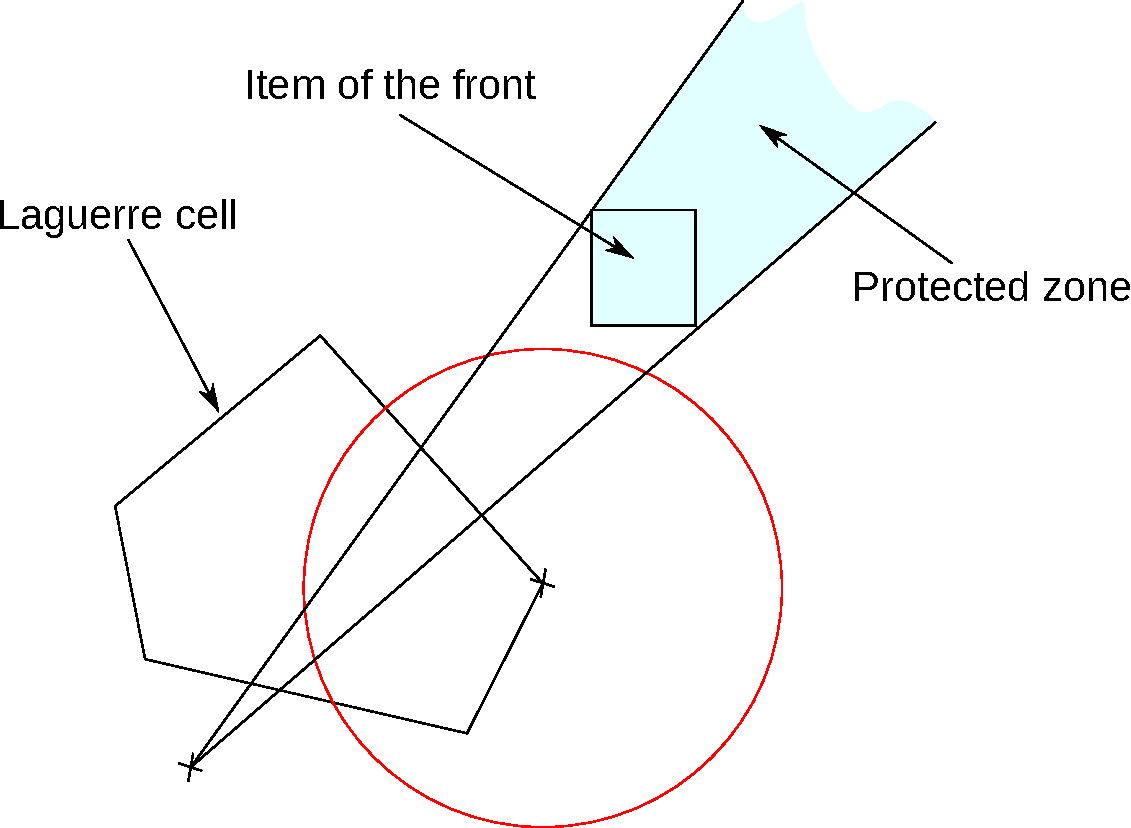
\includegraphics[width=\textwidth]{img/front.pdf}
        \end{center}
    \end{minipage}
    \kern 0.01\textwidth
    \begin{minipage}[c][0.6\textheight][c]{0.35\textwidth}
        \begin{itemize}
            \item Front of boxes are stored in a heap (by distance to the dirac)
            \item Neighbors of a boxes are added to the heap only if possible to find a cutting dirac in the "protected zone"
        \end{itemize}

        \vfill
        \begin{itemize}
            \item Best $\#$ cell / box $\approx$ 20
        \end{itemize}
    \end{minipage}
\end{frame}

\begin{frame}
    \frametitle{Performance, uniform distribution 2D (Voronoï)}

    \begin{minipage}[c][0.6\textheight][c]{0.55\textwidth}
        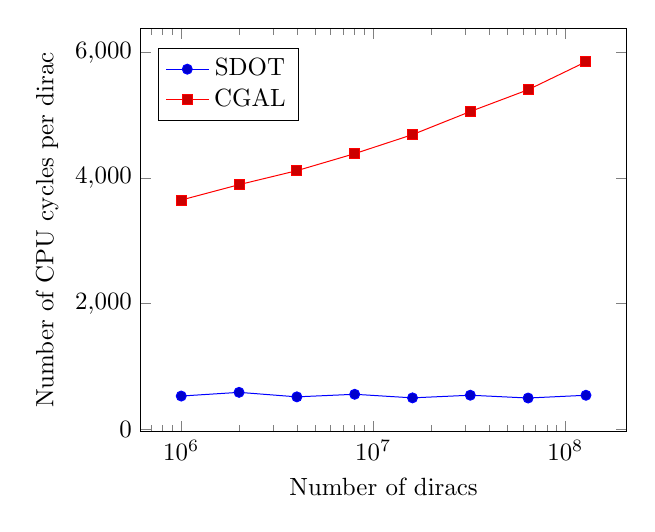
\begin{tikzpicture}[scale=0.9]
    \begin{axis}[
        xmode = log,
        legend style={at={(0.18,0.95)},anchor=north},
        % legend style={at={(0.7,0.4)},anchor=north},
        % ybar interval=0.8,
        xlabel=Number of diracs,
        ylabel=Number of CPU cycles per dirac,
        % enlargelimits=0.05,
    ]
    \addplot coordinates {
       ( 1000000, 528.405 )
       ( 2000000, 587.365 )
       ( 4000000, 515.478 )
       ( 8000000, 556.51 )
       ( 16000000, 499.444 )
       ( 32000000, 541.557 )
       ( 64000000, 496.951 )
       ( 128000000, 540.808 )
    };
    \addplot coordinates {
       ( 1000000, 3650 ) % 2330011341
       ( 2000000, 3895 ) % 3112113216
       ( 4000000, 4118 ) % 2510926143
       ( 8000000, 4389 ) % 4074480963
       ( 16000000, 4692 ) % 3223318630
       ( 32000000, 5060 ) % 558845166
       ( 64000000, 5407 ) % 4192322438
       ( 128000000, 5852 ) % 105099164
    };
    \legend{SDOT, CGAL}
    \end{axis}
\end{tikzpicture}

    \end{minipage}
    \begin{minipage}[c][0.6\textheight][c]{0.4\textwidth}
        \begin{itemize}
            \item Between $7\times$ and $12\times$ speedup

            \bigskip
            \item Almost linear

            \bigskip
            \item Uses a fraction of the memory

            \vfill
            \item Surely not a fair test
        \end{itemize}
    \end{minipage}
\end{frame}


\begin{frame}
    \frametitle{Performance, Voronoï faces distribution 2D (Voronoï)}

    \begin{minipage}[c][0.6\textheight][c]{0.55\textwidth}
        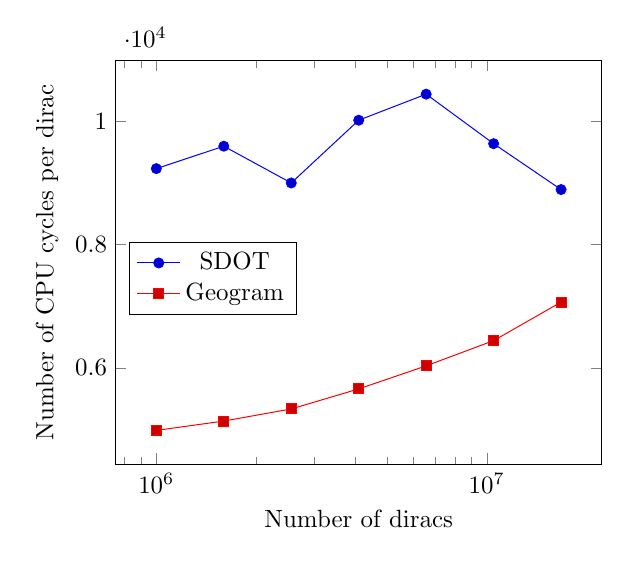
\begin{tikzpicture}[scale=0.9]
    \begin{axis}[
        xmode = log,
        legend style={at={(0.2,0.55)},anchor=north},
        % legend style={at={(0.7,0.4)},anchor=north},
        % ybar interval=0.8,
        xlabel=Number of diracs,
        ylabel=Number of CPU cycles per dirac,
        % enlargelimits=0.05,
    ]
    % SDOT
    \addplot coordinates {
        ( 1000000 , 9232.23 )
        ( 1600000 , 9595.59 )
        ( 2560000 , 8999.55 )
        ( 4096000 , 10017   )
        ( 6553600 , 10439.3 )
        ( 10485760, 9636.75 )
        ( 16777216, 8892.48 )
    };
    % Geogram
    \addplot coordinates {
        ( 1000000, 4987 ) % 7.08315e+06
        ( 1600000, 5139 ) % 1.32546e+07
        ( 2560000, 5335 ) % 1.93817e+07
        ( 4096000, 5660 ) % 2.36147e+07
        ( 6553600, 6034 ) % 3.91585e+07
        ( 10485760, 6443 ) % 5.69583e+07
        ( 16777216, 7067 ) % 9.2984e+07
        % ( 26843545, 7828 ) % 1.64099e+08
    };
    \legend{SDOT, Geogram}
    \end{axis}
\end{tikzpicture}

    \end{minipage}
    \begin{minipage}[c][0.6\textheight][c]{0.4\textwidth}
        \begin{itemize}
            \item A very naughty case

            \bigskip
            \item Good scalability (CPU and memory)
        \end{itemize}
    \end{minipage}
\end{frame}

% \begin{frame}
%     \frametitle{Performance, uniform distribution 3D (Voronoï)    TODO}

%     \begin{minipage}[c][0.6\textheight][c]{0.55\textwidth}
%         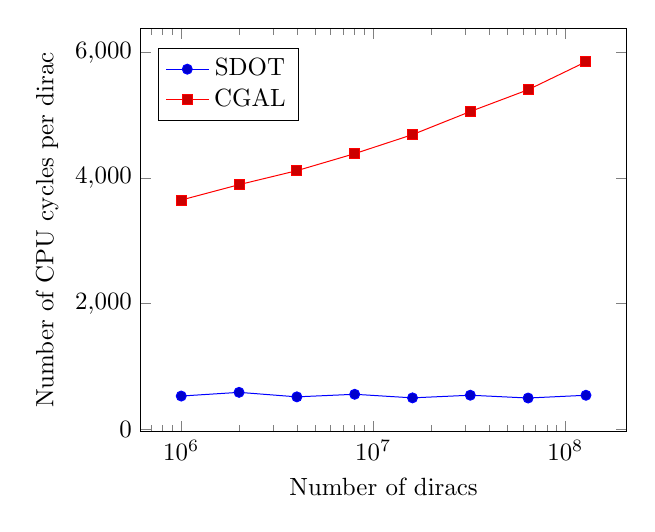
\begin{tikzpicture}[scale=0.9]
    \begin{axis}[
        xmode = log,
        legend style={at={(0.18,0.95)},anchor=north},
        % legend style={at={(0.7,0.4)},anchor=north},
        % ybar interval=0.8,
        xlabel=Number of diracs,
        ylabel=Number of CPU cycles per dirac,
        % enlargelimits=0.05,
    ]
    \addplot coordinates {
       ( 1000000, 528.405 )
       ( 2000000, 587.365 )
       ( 4000000, 515.478 )
       ( 8000000, 556.51 )
       ( 16000000, 499.444 )
       ( 32000000, 541.557 )
       ( 64000000, 496.951 )
       ( 128000000, 540.808 )
    };
    \addplot coordinates {
       ( 1000000, 3650 ) % 2330011341
       ( 2000000, 3895 ) % 3112113216
       ( 4000000, 4118 ) % 2510926143
       ( 8000000, 4389 ) % 4074480963
       ( 16000000, 4692 ) % 3223318630
       ( 32000000, 5060 ) % 558845166
       ( 64000000, 5407 ) % 4192322438
       ( 128000000, 5852 ) % 105099164
    };
    \legend{SDOT, CGAL}
    \end{axis}
\end{tikzpicture}

%     \end{minipage}
%     \begin{minipage}[c][0.6\textheight][c]{0.4\textwidth}
%         \begin{itemize}
%             \item ...
%         \end{itemize}
%     \end{minipage}
% \end{frame}


% \begin{frame}
%     \frametitle{Performance, Voronoï distribution 3D (Voronoï)    TODO}
    
%     \begin{minipage}[c][0.6\textheight][c]{0.55\textwidth}
%         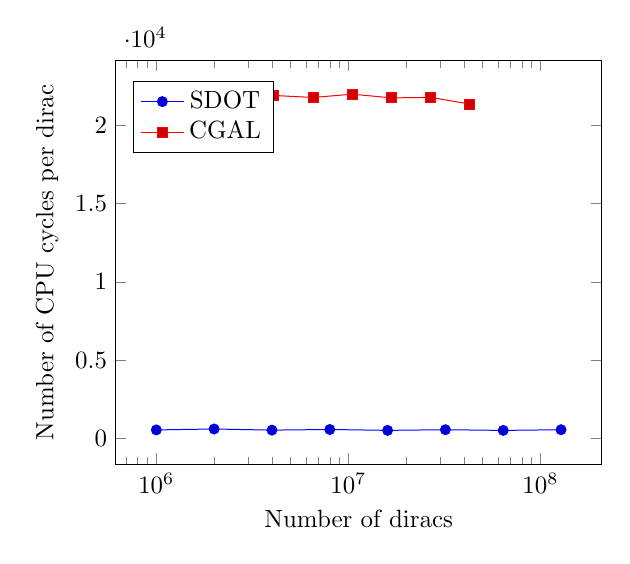
\begin{tikzpicture}[scale=0.9]
    \begin{axis}[
        xmode = log,
        legend style={at={(0.18,0.95)},anchor=north},
        % legend style={at={(0.7,0.4)},anchor=north},
        % ybar interval=0.8,
        xlabel=Number of diracs,
        ylabel=Number of CPU cycles per dirac,
        % enlargelimits=0.05,
    ]
    \addplot coordinates {
       ( 1000000, 528.405   )
       ( 2000000, 587.365   )
       ( 4000000, 515.478   )
       ( 8000000, 556.51    )
       ( 16000000, 499.444  )
       ( 32000000, 541.557  )
       ( 64000000, 496.951  )
       ( 128000000, 540.808 )
    };
    \addplot coordinates {
       ( 1000000  , 21604 )
       ( 1600000  , 21652 )
       ( 2560000  , 21720 )
       ( 4096000  , 21912 )
       ( 6553600  , 21782 )
       ( 10485760 , 21994 )
       ( 16777216 , 21756 )
       ( 26843545 , 21789 )
       ( 42949672 , 21359 )
    };
    \legend{SDOT, CGAL}
    \end{axis}
\end{tikzpicture}

%     \end{minipage}
%     \begin{minipage}[c][0.6\textheight][c]{0.4\textwidth}
%         \begin{itemize}
%             \item ...
%         \end{itemize}
%     \end{minipage}
% \end{frame}

\begin{frame}
    \frametitle{For heterogeneous Kantorovich potentials}

    \begin{minipage}[c][0.7\textheight][c]{0.45\textwidth}
        Quadtree / octree, upper bounds:
        \begin{itemize}
            \item for each dirac,
            \item starting with a paving heap,
            \item while the heap is not empty,
            \item \ \kern 2mm take the top,
            \item \ \kern 2mm if potential cut, go inside,
            \item \ \kern 2mm and place sub-cells in the heap.
        \end{itemize}
    \end{minipage}
    \kern 0.04\textwidth
    \begin{minipage}[c][0.7\textheight][c]{0.5\textwidth}
        \begin{center}
            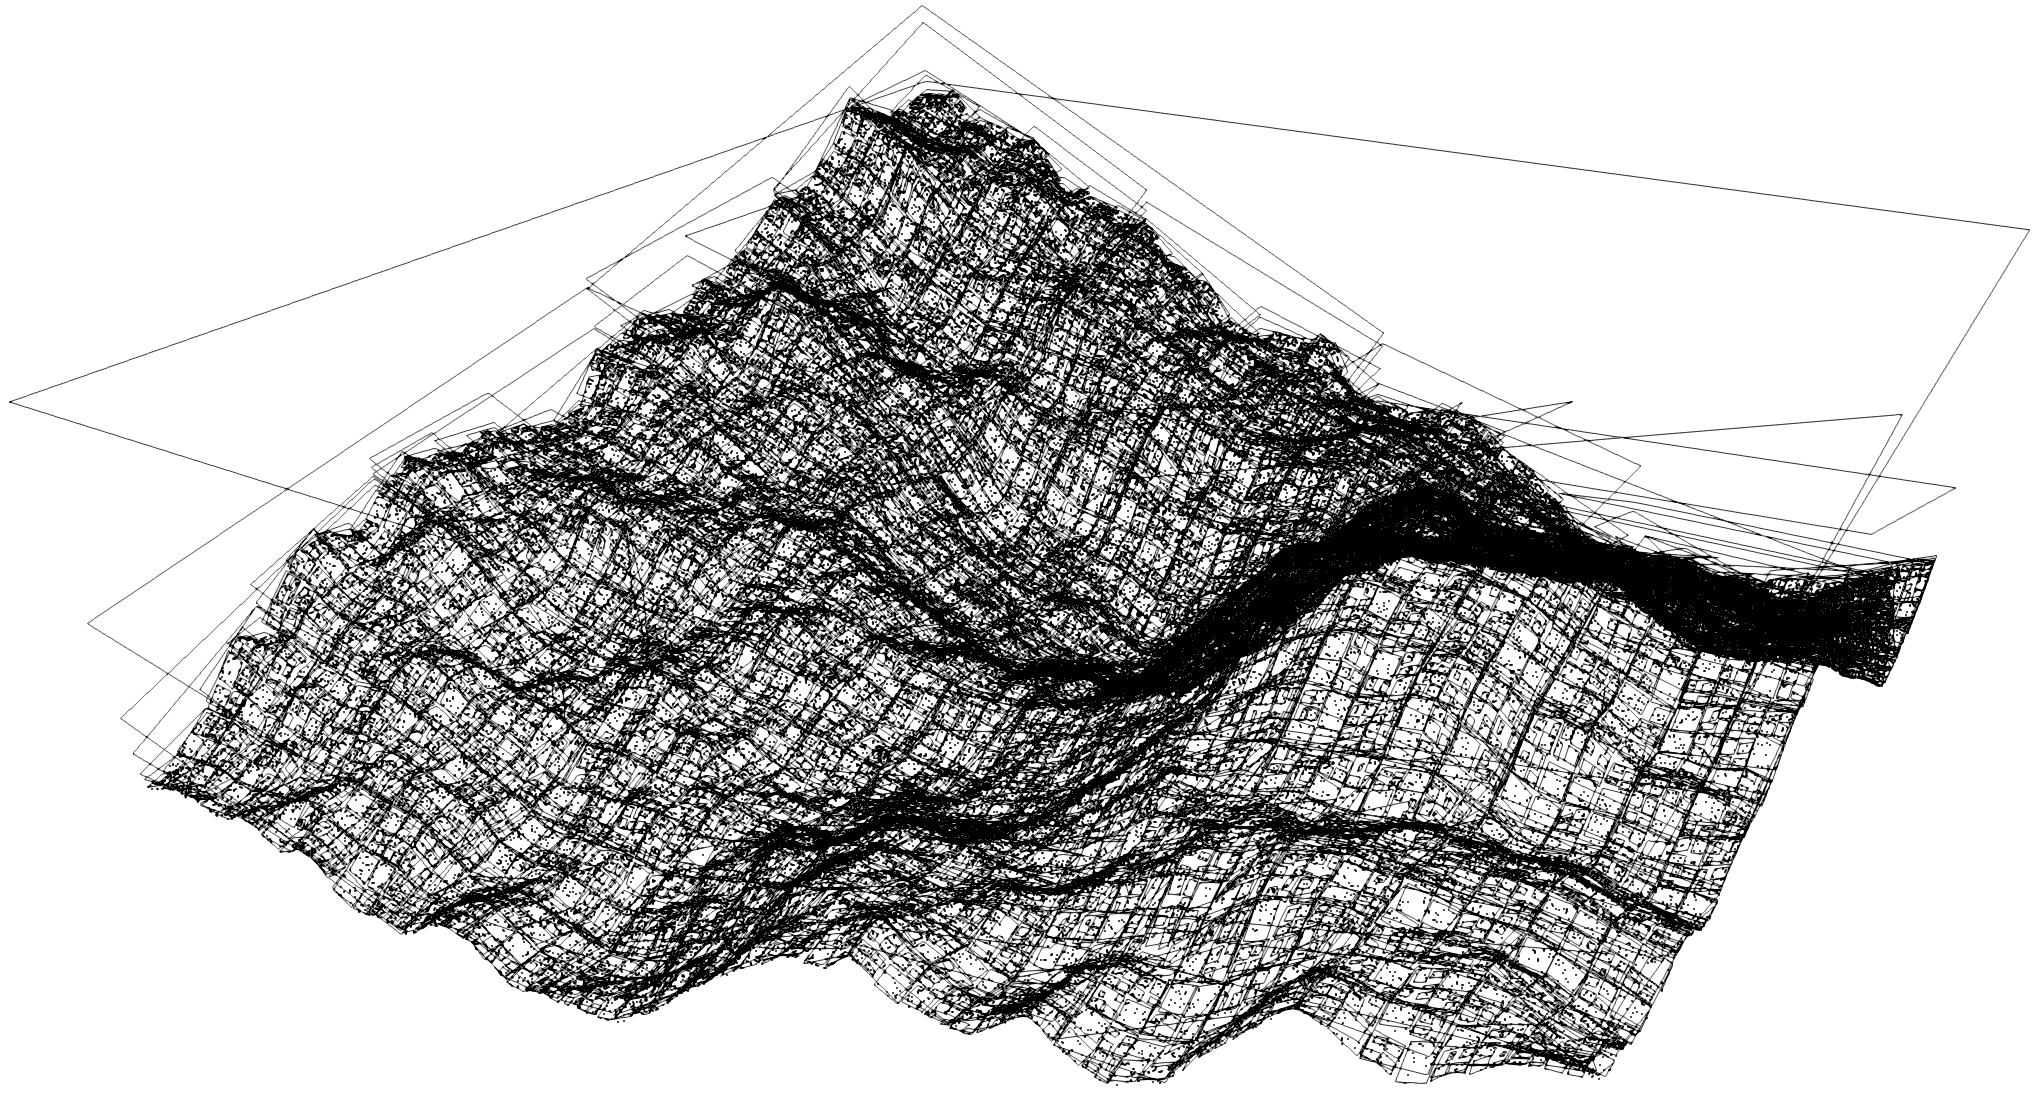
\includegraphics[width=\textwidth]{img/bound_p1.png}

            With upper bounds of degree 1
        \end{center}
    \end{minipage}
\end{frame}

\begin{frame}
    \frametitle{For heterogeneous Kantorovich potentials}

    Remarks:
    \begin{itemize}
        \item closed forms for degree 2 are easy to obtain but come with a high computation cost.
        \item $\mathcal{O}( n \log{} n )$ ops but $\mathcal{O}( n )$ RAM reads
        \item optimal $\#$ dirac per box $\approx$ 30.
    \end{itemize}
\end{frame}


\begin{frame}
    \frametitle{Performance, uniform distribution 2D (optimal weights)}

    \begin{minipage}[c][0.6\textheight][c]{0.55\textwidth}
        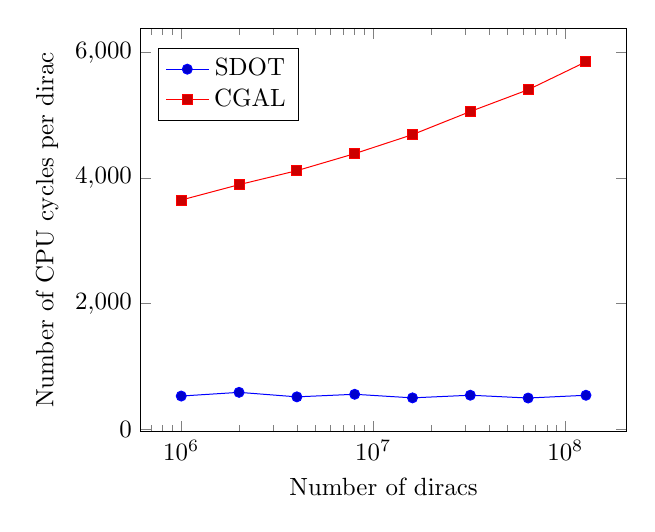
\begin{tikzpicture}[scale=0.9]
    \begin{axis}[
        xmode = log,
        legend style={at={(0.18,0.95)},anchor=north},
        % legend style={at={(0.7,0.4)},anchor=north},
        % ybar interval=0.8,
        xlabel=Number of diracs,
        ylabel=Number of CPU cycles per dirac,
        % enlargelimits=0.05,
    ]
    \addplot coordinates {
       ( 1000000, 528.405 )
       ( 2000000, 587.365 )
       ( 4000000, 515.478 )
       ( 8000000, 556.51 )
       ( 16000000, 499.444 )
       ( 32000000, 541.557 )
       ( 64000000, 496.951 )
       ( 128000000, 540.808 )
    };
    \addplot coordinates {
       ( 1000000, 3650 ) % 2330011341
       ( 2000000, 3895 ) % 3112113216
       ( 4000000, 4118 ) % 2510926143
       ( 8000000, 4389 ) % 4074480963
       ( 16000000, 4692 ) % 3223318630
       ( 32000000, 5060 ) % 558845166
       ( 64000000, 5407 ) % 4192322438
       ( 128000000, 5852 ) % 105099164
    };
    \legend{SDOT, CGAL}
    \end{axis}
\end{tikzpicture}

    \end{minipage}
    \begin{minipage}[c][0.6\textheight][c]{0.4\textwidth}
        \begin{itemize}
            \item $\approx 3 \times$ speedup

            \bigskip
            \item Almost linear

            \bigskip
            \item Uses a fraction of the memory
        \end{itemize}
    \end{minipage}
\end{frame}

\begin{frame}
    \frametitle{Performance, uniform distribution 3D (optimal weights)}

    \begin{minipage}[c][0.6\textheight][c]{0.55\textwidth}
        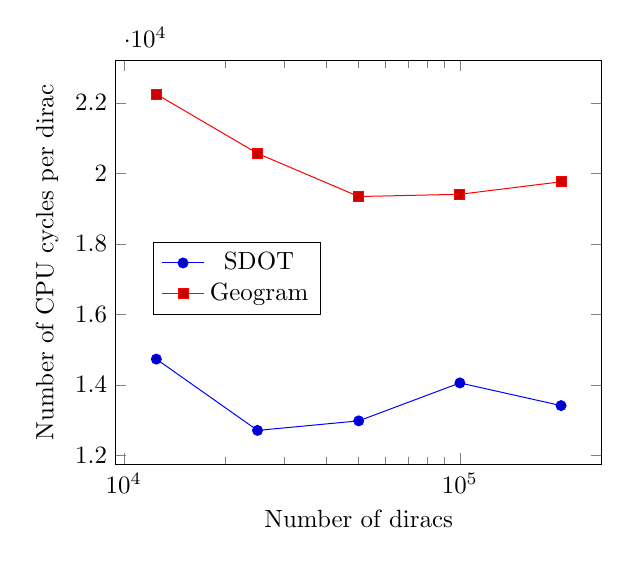
\begin{tikzpicture}[scale=0.9]
    \begin{axis}[
        xmode = log,
        legend style={at={(0.25,0.55)},anchor=north},
        % legend style={at={(0.7,0.4)},anchor=north},
        % ybar interval=0.8,
        xlabel=Number of diracs,
        ylabel=Number of CPU cycles per dirac,
        % enlargelimits=0.05,
    ]
    \addplot coordinates {
        ( 12500 , 14729 )
        ( 25000 , 12705 )
        ( 50000 , 12976 )
        ( 100000, 14052 )
        ( 200000, 13409 )
    };
    \addplot coordinates {
        ( 12500 , 22247 ) % 2.51726e+07
        ( 25000 , 20565 ) % 5.03384e+07
        ( 50000 , 19342 ) % 1.00954e+08
        ( 100000, 19406 ) % 2.01818e+08
        ( 200000, 19761 ) % 4.04263e+08
    };
    \legend{SDOT, Geogram}
    \end{axis}
\end{tikzpicture}

    \end{minipage}
    \begin{minipage}[c][0.6\textheight][c]{0.4\textwidth}
        \begin{itemize}
            \item $\approx 1.5 \times$ speedup
            
            \bigskip{}
            \item (more optimizations to come)
        \end{itemize}
    \end{minipage}
\end{frame}

\begin{frame}
    \frametitle{Distributed memory, out-of-core}

    \begin{minipage}[c][0.6\textheight][c]{0.5\textwidth}
        Replicated storage of a portion of the acceleration structure.

        \bigskip
        Handling of lists of unfinished cells + prefetching (immediate neighbors).

        \vfill
        Done in 1 step for most cases.
    \end{minipage}
    \kern 0.04\textwidth 
    \begin{minipage}[c][0.6\textheight][c]{0.4\textwidth}
        \begin{center}
            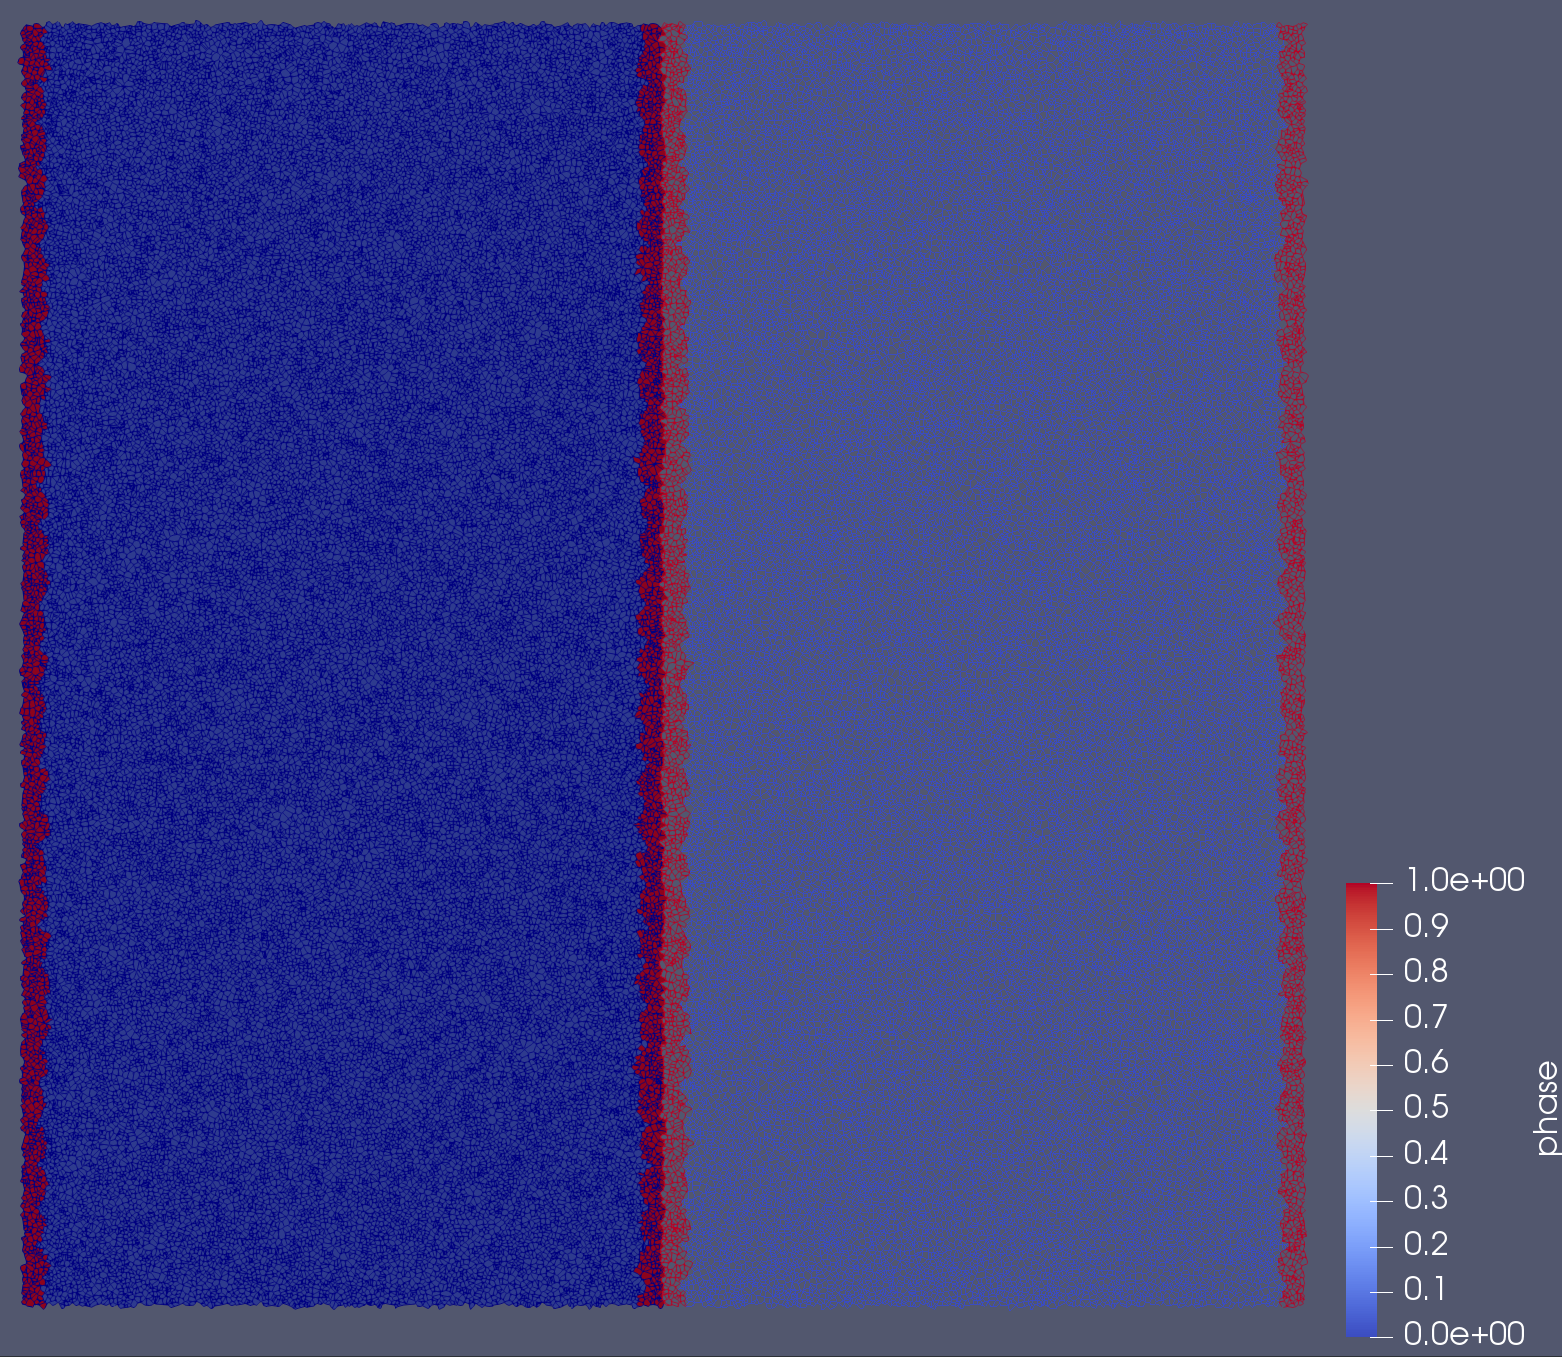
\includegraphics[width=\textwidth]{img/mpi.png}
            
            MPI/out-of core Phase number \\ (without prefetching)
        \end{center}
    \end{minipage}
\end{frame}


% ---------------------------------------------------------------------------------------
\section{Product placement}

\begin{frame}[fragile]
    \frametitle{SDOT, PySDOT}

    \begin{minipage}[c][0.8\textheight][c]{0.44\textwidth}
        Packaged in a library, with examples
        \begin{itemize}
            \item github, pip, conda (precompiled)
            \item pythonic bindings
        \end{itemize}
    
        \vfill        
        Integration
        \begin{itemize}
            \item Radial functions: \\ $1$, $|x|^2$, $|x| < r$, $e^{-x^2 / \tau}$, ...
            \item Space functions: \\ on polyhedra, from an image ($\mathcal{O}( max( m, n ) )$)...
            \item Der. wrt KP \& positions
        \end{itemize}
    
        \vfill
        Geometry
        \begin{itemize}
            \item Periodicity (affine trans.), etc...
        \end{itemize}
    \end{minipage}
    \begin{minipage}[c][0.8\textheight][c]{0.55\textwidth}
        \begin{scriptsize}
            \begin{lstlisting}[language=Python]
from pysdot.domain_types import ScaledImage
from pysdot import OptimalTransport

ot = OptimalTransport(
    positions = np.rand.random( 100, 2 ),
    domain = ScaledImage( [0, 0], [1, 1], ... )
    radial_function = ...
)

ot.adjust_weights()

print( ot.get_centroids() )
print( ot.second_order_moments() )
print( ot.img_integrals( [ 100, 100 ] ) )
print( ot.der_centroids_and_integrals_wrt_
          weight_and_positions() )
...
            \end{lstlisting}
        \end{scriptsize}
    \end{minipage}
\end{frame}

\begin{frame}
    \frametitle{Some applications}

    \begin{minipage}[c][0.8\textheight][c]{0.4\textwidth}
        \begin{center}
            
\includegraphics[width=\textwidth]{img/pd_002.pdf}

            2D congestion flow

            \vfill
            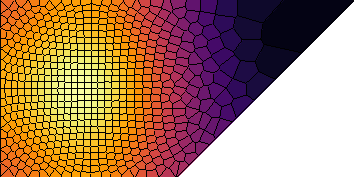
\includegraphics[width=\textwidth]{img/pd_003.pdf}

            Diffusion
        \end{center}
    \end{minipage}
    \begin{minipage}[c][0.8\textheight][c]{0.55\textwidth}
        \begin{center}
            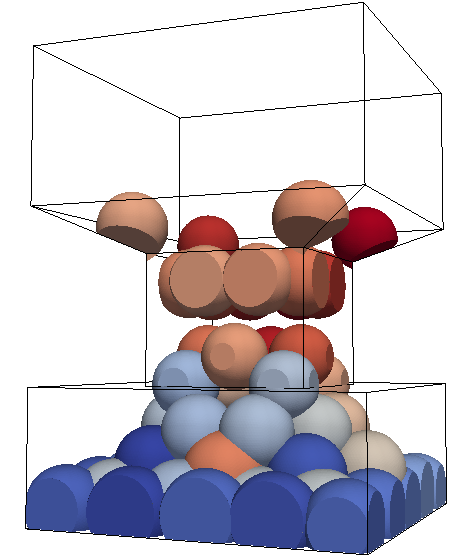
\includegraphics[width=0.7\textwidth]{img/pd_004.png}

            3D congestion flow
        \end{center}
    \end{minipage}
\end{frame}

% ---------------------------------------------------------------------------------------
\section{Wrap up}

\begin{frame}
    \frametitle{Conclusions}

    Cell centered algorithms:
    \begin{itemize}
        \item good performance
        \item with a fraction of the memory
        \item parallel by default, with strong scaling
    \end{itemize}
    
    \vfill
    Acceleration structures:
    \begin{itemize}
        \item mostly $\mathcal{O}( n )$ for construction and traversal
        \item fits well the tested cases
    \end{itemize}
\end{frame}

\begin{frame}
    \frametitle{Perspectives}

    Optimizations
    \begin{itemize}
        \item Better bounds for the Kantorovich potentials
        \item More SIMD optimizations for the 3D case
        \item GPU
    \end{itemize}

    \vfill
    Solvers
    \begin{itemize}
        \item preconditioners
        \item multi-grid
    \end{itemize}
\end{frame}

\end{document}
